\chapter{Experimente}\label{ch:experiments}
In diesem Kapitel werden wir drei verschiedene Beispiele mit sämtliche eingeführten Methoden berechnen. Dabei wird zunächst auf die Lösung der Differentialgleichung eingegangen und es werden Konvergenzbetrachtungen durchgeführt. Danach erfolgt die Berechnung des Gradienten des Kostenfunktionals und die Optimierung für diverse Anfangswerte.

Als erstes Problem dient das Rolling Stones Beispiel, welche ein stückweise lineares Problem darstellt. 
Das darauf folgende Beispiel, die LC-Diode, ist ein System von gewöhnlichen Differentialgleichungen, welche nahe der Maschinengenauigkeit modellieren. Als Abschluss wird die 1-D Shallow Water Equation ortsdiskretisiert, sodass sie mit der verallgemeinerten Mittelpunktsregel als System von ODEs in der Zeit gelöst werden kann. Im Folgenden werden wir mit \glqq IMP\grqq~die klassische implizite Mittelpunktsregel und mit \glqq GIMP\grqq~die verallgemeinerte implizite Mittelpunktsregel bezeichnen.

\section{Rolling Stone}\label{sec:rollingStonesExample}
% \subsection{Problemstellung}
Zum Anfang wollen wir uns dem sogenannten Rolling Stones Beispiel widmen, welches beispielsweise in \cite{boeck2014experiments} oder \cite{hasenfelder13} eingeführt wurde. 
Es behandelt eine sich reibungslos bewegende Kugel auf einer konvexen Parabel, in dessen Mitte eine flache Ebene auf dem Intervall $[-1,1]$ eingefügt wurde. 
\begin{figure}[ht]
\centering
\begin{minipage}[b]{0.49\linewidth}
% \begin{minipage}[t][3cm][t]{5cm}
\documentclass{standalone}
\IfStandalone{
	\usepackage{pgfplots,pgfplotstable}
	\usetikzlibrary{external}
	
	}{%
}
% \usepackage{pgfplots,pgfplotstable}
% \usetikzlibrary{external}
	

\begin{document}
\tikzsetnextfilename{rolling-stones}
\begin{tikzpicture}[x=3em,y=3em]
\begin{axis}[
            xmin=-2.5,xmax=2.5,
            ymin=-1.5,ymax=1.5,
            xlabel=$z$,
%             legend entries={$V(z)$,$V'(z)$},
            width=\linewidth
        ]
        \addplot[domain=-2.5:-1]{(1+x)^2/2};
        \addplot[-,domain=-1:1]{0};
        \addplot[domain=1:2.5]{(1-x)^2/2};
        \addplot[domain=-2.5:2.5,samples=100,blue]{-min(max(-1-x,0),1-x)};
\end{axis}
\end{tikzpicture}

 
\end{document}

\caption{Rolling Stones}
\label{fig:rollingStones}
\end{minipage}
% \quad
\begin{minipage}[b]{0.49\linewidth}
% \begin{minipage}[t][3cm][t]{5cm}
\documentclass{standalone}
\IfStandalone{
	\usepackage{pgfplots,pgfplotstable}
	\usetikzlibrary{external}
	
	}{%
}
\begin{document}
\tikzsetnextfilename{rolling-stones-solution}
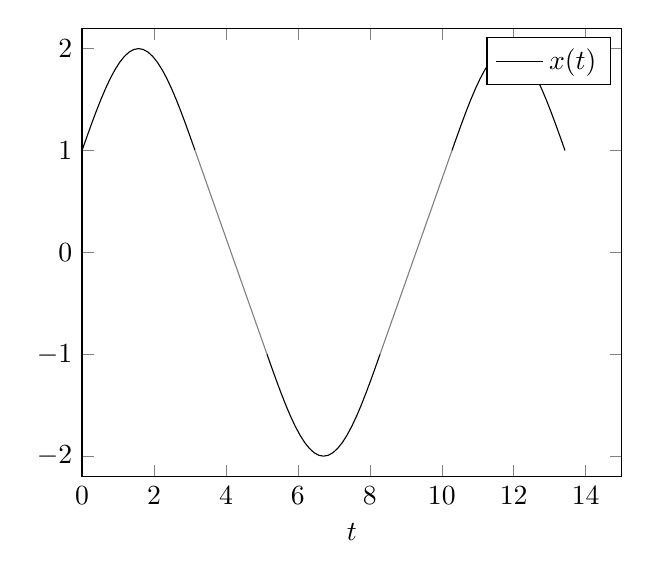
\begin{tikzpicture}[x=3em,y=3em]
\begin{axis}[
            xmin=0,xmax=15,
            ymin=-2.2,ymax=2.2,
            xlabel=$t$,
            legend entries={$x(t)$}
        ]
        \addplot[domain=0:3.14]{1+sin(deg(x))};
        \addplot[domain=pi:pi+2,gray]{1-x+pi};
        \addplot[domain=pi+2:2*pi+2]{-1-sin(deg(2-x))};
        \addplot[domain=2*pi+2:2*pi+4,gray]{x-3-2*pi};
        \addplot[domain=2*pi+4:3*pi+4]{1+sin(deg(x-2*pi-4))};
\end{axis}
\end{tikzpicture} 
\end{document}

\caption{Rolling Stones Lösung}
\label{fig:rollingStonesSolution}
\end{minipage}
\end{figure}
Abbildung \ref{fig:rollingStones} zeigt die Rampe
\[
 V(z) = \left(\frac{(1+z)^2}{2}\right)\chi_{(-\infty,-1]} + \left(\frac{(1-z)^2}{2}\right)\chi_{[1,\infty)} ,
 ~ \chi_{[a,b)}(z) = 
 \begin{cases}
  1 & z \in [a,b)\\
  0 & \text{sonst}
 \end{cases}
\]

und deren Ableitung, welche hier als gewöhnliche Differentialgleichung
 \begin{equation}
  \begin{pmatrix}
   \dot x_1 \\
   \dot x_2 \\
  \end{pmatrix}
 = 
 \begin{pmatrix}
  x_2 \\
  -x_1 - \frac{|x_1-1|}{2} + \frac{|x_1+1|}{2}
 \end{pmatrix}
=F(x)
\label{eq:rolling_stones}
 \end{equation}
aufgefasst wird. Die Variable $x_1$ bezeichnet die Abszissenposition des Steines und $x_2$ dessen Geschwindigkeit.
Die Funktion \eqref{eq:rolling_stones} ist stückweise linear, sodass wir seine Abs-Normal Form \eqref{eq:absNormalForm} angeben können:
\[
c = \begin{pmatrix}
     -1\\
     1
    \end{pmatrix}
\quad
 Z = \begin{pmatrix}
      1 & 0 \\
      1 & 0
     \end{pmatrix}\quad
J = \begin{pmatrix}
      0&1\\
      -1 & 0
     \end{pmatrix}\quad
 Y = \begin{pmatrix}
      0 & 0\\
      -0.5  & 0.5
     \end{pmatrix}.
\]
Der Rest wird passend zur Dimension zu $0$ gesetzt. Für das Rolling Stones Beispiel lässt sich eine analytische Lösung zur ODE \eqref{eq:rolling_stones} für den Anfangswert $x_0=(1,1)$ angeben. Sie ist $2\pi+4$ periodisch, hat die Form
\begin{equation}
 x(t) = \begin{cases}
         1+\sin(t) 	& 0\leq t \leq \pi	\\
         1-(t-\pi) 	& \pi \leq t < \pi+2	\\ 
         -1 - \sin(2-t) 	& \pi+2\leq t<2\pi+2	\\
         t-3-2\pi	& 2\pi+2 \leq t<2\pi +4
        \end{cases}
\label{eq:analyticSolRolling}
\end{equation}
und wird in Abbildung \ref{fig:rollingStonesSolution} gezeigt. Dabei sind die grau eingezeichneten Bereiche linear.

\subsection{Lösen der ODE}
% Die Konvergenz der verallgemeinerten impliziten Mittelpunktsregel 
\begin{figure}
\centering
\documentclass{standalone}
\IfStandalone{
	\usepackage{pgfplots,pgfplotstable}
	\usetikzlibrary{external}
	\newcommand{\fromRoot}[1]{../#1}
}{%
}
\begin{document}
\tikzsetnextfilename{convergence_rolling_plot}
\begin{tikzpicture}
\begin{loglogaxis}[
	width=10cm,
	xlabel=Degrees of freedom $N$,
	ylabel=Error at time $T$,
	legend entries ={Expl. MP,
	IMP,
	GIMP, 
	}
]
  	\addplot[mark=none,red,very thin] table[x index=0,y index=2] {img/data/convergence_rolling_plot.dat};%expl midpoint
 	\addplot[mark=none,green,very thin] table[x index=0,y index=3] {img/data/convergence_rolling_plot.dat};%impl midpoint
	\addplot[mark=none,blue,very thin] table[x index=0,y index=1] {img/data/convergence_rolling_plot.dat};%gen midpoint

	\addplot[mark=none,very thin,gray, yshift=-20pt] 
		table[y={create col/linear regression={x=0,y=1}}] {img/data/convergence_rolling_plot.dat}
		  coordinate [pos=0.5] (A)
		  coordinate [pos=0.6] (B)
		;
	% save the slope parameter:
	\pgfmathparse{-\pgfplotstableregressiona}	
	\pgfmathsetmacro{\slope}{\pgfmathresult}
	
	% draw the opposite and adjacent sides
	% of the triangle
	\draw[very thin,gray] (B) -| (A)
	node [pos=0.2,anchor=north]
	{\pgfmathprintnumber{\slope}};
\end{loglogaxis}
\end{tikzpicture}
\end{document}
\caption{Konvergenz Rolling Stones im Intervall $[0,50]$ mit $x_0=(1,1)$}
\label{fig:rollingStonesConvergence}
\end{figure}


\begin{figure}[H]
\footnotesize 
\centering
% \quad
\begin{minipage}[b]{0.45\linewidth}
% \begin{minipage}[t][3cm][t]{5cm}
\documentclass{standalone}
\IfStandalone{
	\usepackage{pgfplots,pgfplotstable}
	\usetikzlibrary{external}
	\newcommand{\fromRoot}[1]{../#1}
}{%
}

\begin{document}
\tikzsetnextfilename{rolling_energy_error}
\begin{tikzpicture}
\begin{loglogaxis}[
	width=\linewidth,
	xlabel=Anzahl der Freiheitsgrade $N$,
	ylabel=Mittelwert des Energieverlustes,
	legend entries ={Expl. MP,
	IMP,
	GIMP 
	},
	legend style={at={(0.5,1.0)},anchor=south},
	legend columns=2
]
  	\addplot[mark=none,red,very thin] table[x index=0,y index=2] {\fromRoot img/data/rolling_energy_error.dat};%expl midpoint
 	\addplot[mark=none,green,very thin] table[x index=0,y index=3] {\fromRoot img/data/rolling_energy_error.dat};%impl midpoint
	\addplot[mark=none,blue,very thin] table[x index=0,y index=1] {\fromRoot img/data/rolling_energy_error.dat};%gen midpoint
\end{loglogaxis}
\end{tikzpicture}
\end{document}
\caption{Rolling Stones Energieverlust im Intervall $[0,2\pi+4]$ mit $x_0=(1,1)$}
\label{fig:rollingStonesEnergyError}
\end{minipage}
\quad
\begin{minipage}[b]{0.45\linewidth}
% \begin{minipage}[t][3cm][t]{5cm}
\documentclass{standalone}
\IfStandalone{
	\usepackage{pgfplots,pgfplotstable}
	\usetikzlibrary{external}
	\newcommand{\fromRoot}[1]{../#1}
}{%
}
\begin{document}
\tikzsetnextfilename{convergence_rolling_romberg_plot}
\begin{tikzpicture}
\begin{loglogaxis}[
	width=10cm,
	xlabel=Anzahl der Freiheitsgrade $N$,
	ylabel=Fehler in $x$,
% 	title=Convergence of SWE,
	legend entries ={
% 	Expl. MP,
	IMP,
	GIMP, 
	Romberg Impl,
	Romberg Gen
	}
]
 	\addplot[mark=none,green,very thin] table[x index=0,y index=3] {img/data/convergence_rolling_romberg_plot.dat};%impl midpoint
	\addplot[mark=none,blue,very thin] table[x index=0,y index=1] {img/data/convergence_rolling_romberg_plot.dat};%gen midpoint

	\addplot[mark=none,lime,very thin] table[x index=0,y index=5] {img/data/convergence_rolling_romberg_plot.dat};%Romberg impl midpoint
	\addplot[mark=none,cyan,very thin] table[x index=0,y index=4] {img/data/convergence_rolling_romberg_plot.dat};%ROMBERG gen midpoint
	
	
	\addplot[mark=none,very thin,gray, yshift=-20pt] 
		table[y={create col/linear regression={x=0,y=4}}] {img/data/convergence_rolling_romberg_plot.dat}
		  coordinate [pos=0.5] (A)
		  coordinate [pos=0.6] (B)
		;
	% save the slope parameter:
	\pgfmathparse{-\pgfplotstableregressiona}	
	\pgfmathsetmacro{\slope}{\pgfmathresult}
	
	% draw the opposite and adjacent sides
	% of the triangle
	\draw[very thin,gray] (B) -| (A)
	node [pos=0.2,anchor=north]
	{\pgfmathprintnumber{\slope}};
\end{loglogaxis}
\end{tikzpicture}
\end{document}
\caption{Romberg Konvergenz im Intervall $[0,50]$ mit $x_0=(1,1)$}
\label{fig:rollingStonesConvergenceRomberg}
\end{minipage}

\end{figure}


Die in Theorem \ref{thm:convergenceGenMidpoint} vorhergesagte Konvergenzordnung von $\mathcal O(h^2)$ erfüllt die GIMP wie in Abbildung \ref{fig:rollingStonesConvergence} ersichtlich ist.
Dass die IMP eine ebenso hohe Konvergenzrate besitzt, liegt darin begründet, dass sie im gegebenen Intervall nur $4$ mal pro $2\pi+4$ Periode Unglattheiten überquert, sonst jedoch normal konvergiert. Aufgrund dieser Unglattheiten entsteht für die IMP kein glatter Konvergenzgraph, sondern sie springt. Demgegenüber konvergiert die GIMP sehr stabil, da sie die Kinks der Funktion mit in ihre Berechnung einbezieht.
Insbesondere wird der Fehler der GIMP mit zunehmender Zeit (siehe Fig. \ref{fig:rollingStonesEOT}(a)) nur in den nicht affinen Abschnitten größer, währenddessen in den affinen Abschnitten exakt gelöst wird. Der lokale Fehler der IMP erhöht sich jedoch ständig, bedingt durch die Kinks und der zu großen Schrittweite. Der allgemeine Fehler ist dadurch für die IMP größer im zeitlichen Verlauf, als der Fehler der GIMP (\ref{fig:rollingStonesEOT}(b)).

Da sich der rollende Stein reibungslos in unserem System bewegt, muss die analytische Lösung die komplette Energie erhalten, d.h. die Summe der potentiellen und der kinetischen Energie $V(x) + \frac{1}{2}\dot x^2$ muss konstant sein. Die Abbildung \ref{fig:rollingStonesEnergyError} wurde mittels der summierten Variation der Energie 
\begin{equation}
 h \left[\sum_{l=0}^{T/h} \left( V(x_1^l) + \frac{1}{2} (x_2^l)^2 -\frac{1}{2}\right)^2\right]^{\sfrac{1}{2}}
 \label{eq:energyVariation}
\end{equation}
berechnet. Es ist deutlich zu erkennen, dass die Energie mit der GIMP deutlich besser erhalten bleibt als mit den klassischen Methoden, selbst für große Schrittweiten.
Dadurch führt die in Abbildung \ref{fig:rollingStonesConvergenceRomberg} durchgeführte Romberg Extrapolation zu sehr guten Ergebnissen. Da der Konvergenzgraph der GIMP stabil ist, lässt sich eine gute Extrapolation mit Konvergenzen der Ordnung 3 bis 4 erreichen, wie in Theorem \ref{thm:rombergConvergence} vorhergesagt. Demgebenüber besitzt die Extrapolation der IMP keine höhere Konvergenzordnung als die der IMP selbst.
\begin{figure}[H]
\footnotesize 
\centering
\begin{minipage}[b]{0.49\linewidth}
% \begin{minipage}[t][3cm][t]{5cm}
\documentclass{standalone}
\IfStandalone{
	\usepackage{pgfplots,pgfplotstable}
	\usetikzlibrary{external}
	\newcommand{\fromRoot}[1]{../#1}
}{%
}
\begin{document}
\tikzsetnextfilename{rolling_error_over_time}
\begin{tikzpicture}
\begin{axis}[
	width=\linewidth,
	xlabel=Zeitpunkt $t$,
	ylabel=Fehler zum Zeitpunkt $t$,
	legend entries ={Expl. MP,
	IMP,
	GIMP, 
	},
	legend style={at={(0,1)},anchor=north west}
]
\addplot[mark=none,red,very thin] table[x index=0,y index=3] {img/data/rolling_error_over_time.dat};
\addplot[mark=none,green,very thin] table[x index=0,y index=2] {img/data/rolling_error_over_time.dat};
\addplot[mark=none,blue,very thin] table[x index=0,y index=1] {img/data/rolling_error_over_time.dat};

\end{axis}
\end{tikzpicture}
\end{document}
\caption*{(a) Am Zeitpunkt $t$}\end{minipage}
% \quad
\begin{minipage}[b]{0.49\linewidth}
% \begin{minipage}[t][3cm][t]{5cm}
\documentclass{standalone}
\IfStandalone{
	\usepackage{pgfplots,pgfplotstable}
	\usetikzlibrary{external}
	\newcommand{\fromRoot}[1]{../#1}
}{%
}
\begin{document}
\tikzsetnextfilename{rolling_error_over_time_all}
\begin{tikzpicture}
\begin{axis}[
	width=\linewidth,
	xlabel=Zeitpunkt $t$,
	ylabel=Fehler über alle Komponenten,
	legend entries ={Expl. MP,
	IMP,
	GIMP 
	},
% 	legend style={at={(0,1)},anchor=north west}
	legend style={at={(0.5,1.0)},anchor=south},
	legend columns=2
]
\addplot[mark=none,red,very thin] table[x index=0,y index=3] {img/data/rolling_error_over_time_all.dat};
\addplot[mark=none,green,very thin] table[x index=0,y index=2] {img/data/rolling_error_over_time_all.dat};
\addplot[mark=none,blue,very thin] table[x index=0,y index=1] {img/data/rolling_error_over_time_all.dat};

\end{axis}
\end{tikzpicture}
\end{document}
\caption*{(b) Summiert}
\end{minipage}
\caption{Rolling Stones Fehler über Zeit, \\$h=0.1,x_0=(1,1)$}
\label{fig:rollingStonesEOT}

\end{figure}

\subsection{Gradient des Kostenfunktionals}
Ähnliche Ergebnisse wie beim Lösen der ODE erwarten wir für die Integration des inhomogenen adjungierten tangent linear models \eqref{eq:inhAdjEquation}. Falls nicht anders beschrieben, werden im Folgenden immer die exakte Lösung des Rolling Stones Beispiel \eqref{eq:analyticSolRolling} als Obervierungsparameter $x_{\text{obs}}$ mit der selben Diskretisierung verwendet, wie bei der Vorwärtsintegration.

Beim Plot des Gradienten nach Anfangswerten, wie in Abbildung \ref{fig:rollingGrad}, ist zu erkennen, dass der Gradient, berechnet mit der GIMP, ebenfalls stabiler wirkt (Fig. \ref{fig:rollingGrad} (a)), als der Gradient berechnet mit der IMP (Fig. \ref{fig:rollingGrad} (b)). Desweiteren existieren im Letzteren vereinzelt hohe Sprünge, welche durch nicht einbezogene Kinks erklärt werden können (siehe Abbildung \ref{fig:multipleKinksAdjoint}). 
\begin{figure}[H]
\footnotesize 
\centering
\begin{minipage}[b]{0.49\linewidth}
% \begin{minipage}[t][3cm][t]{5cm}
\documentclass{standalone}
\usepackage{pgfplots,pgfplotstable}
\IfStandalone{
	\usepackage{pgfplots,pgfplotstable}
	\usetikzlibrary{external}
	\newcommand{\fromRoot}[1]{../#1}
}{%
}
\begin{document}
\tikzsetnextfilename{rolling_jac_da_gradient1}
\begin{tikzpicture}
    \begin{axis}[view={-20}{60}, grid=both,width=\linewidth,
%      title={$\sfrac{\partial J}{\partial x_0^{(1)}}$},
    xlabel={$x_0^{(0)}$},
    ylabel={$x_0^{(1)}$},
    zlabel={$\sfrac{\partial J}{\partial x_0^{(1)}}$}]
      \addplot3[surf] file {img/data/grad1_gimp.dat};
    \end{axis}
\end{tikzpicture}
\end{document}
% \caption{Rolling Stones Fehler über Zeit}
% \label{fig:rollingGrad1Gimp}
\end{minipage}
% \quad
\begin{minipage}[b]{0.49\linewidth}
% \begin{minipage}[t][3cm][t]{5cm}
\documentclass{standalone}
\IfStandalone{
	\usepackage{pgfplots,pgfplotstable}
	\usetikzlibrary{external}
	\newcommand{\fromRoot}[1]{../#1}
}{%
}
\begin{document}
\tikzsetnextfilename{rolling_jac_da_gradient1_imp}
\begin{tikzpicture}
    \begin{axis}[view={-20}{60}, grid=both,width=\linewidth,
%      title={$\sfrac{\partial J}{\partial x_0^{(1)}}$},
    xlabel={$x_0^{(0)}$},
    ylabel={$x_0^{(1)}$},
    zlabel={$\sfrac{\partial J}{\partial x_0^{(1)}}$}]
      \addplot3[surf] file {\fromRoot img/data/grad1_impl.dat};
    \end{axis}
\end{tikzpicture}
\end{document}
% \caption{Rolling Stones Fehler über alle Komponenten}
% \label{fig:rollingGrad1Imp}
\end{minipage}
\begin{minipage}[b]{0.49\linewidth}
% \begin{minipage}[t][3cm][t]{5cm}
\documentclass{standalone}
\IfStandalone{
	\usepackage{pgfplots,pgfplotstable}
	\usetikzlibrary{external}
	\newcommand{\fromRoot}[1]{../#1}
}{%
}
\begin{document}
\tikzsetnextfilename{rolling_jac_da_gradient2}
  \begin{tikzpicture}
    \begin{axis}[view={-20}{60}, grid=both,width=\linewidth,
%      title={$\sfrac{\partial J}{\partial x_0^{(1)}}$},
    xlabel={$x_0^{(0)}$},
    ylabel={$x_0^{(1)}$},
    zlabel={$\sfrac{\partial J}{\partial x_0^{(1)}}$}]
      \addplot3[surf] file {img/data/grad2_gimp.dat};
      
    \end{axis}
\end{tikzpicture}
\end{document}
% \caption{Ableitung des Kostenfunktional in erster Komponente von Rolling Stones }
% \label{fig:rollingGrad2Gimp}
\caption*{(a) GIMP}
\end{minipage}
% \quad
\begin{minipage}[b]{0.49\linewidth}
% \begin{minipage}[t][3cm][t]{5cm}
\documentclass{standalone}
\IfStandalone{
	\usepackage{pgfplots,pgfplotstable}
	\usetikzlibrary{external}
	\newcommand{\fromRoot}[1]{../#1}
}{%
}
\begin{document}
\tikzsetnextfilename{rolling_jac_da_gradient2_imp}
  \begin{tikzpicture}
    \begin{axis}[view={-20}{60}, grid=both,width=\linewidth,
%      title={$\sfrac{\partial J}{\partial x_0^{(1)}}$},
    xlabel={$x_0^{(0)}$},
    ylabel={$x_0^{(1)}$},
    zlabel={$\sfrac{\partial J}{\partial x_0^{(1)}}$}]
      \addplot3[surf] file {img/data/grad2_impl.dat};
      
    \end{axis}
\end{tikzpicture}
\end{document}
% \caption{Ableitung des Kostenfunktional in erster Komponente von Rolling Stones}
% \label{fig:rollingGrad2Imp}
\caption*{(b) IMP}
\end{minipage}
\caption{Ableitung des Kostenfunktionals beim Rolling Stones Beispiel, $I = [0,30],h=0.5$}
\label{fig:rollingGrad}
\end{figure}

Die Abbildung \ref{fig:rolling_adjoint_eq} zeigt die rückwärts zu integrierende rechte Seite. Dabei sind für die Geschwindigkeit $\dot{\bar{x_2}}$, genau an den Übergängen zu den linearen Teilen der Funktion, Sprünge zu erkennen.
\begin{figure}[H]
\centering
\documentclass{standalone}
\IfStandalone{
	\usepackage{pgfplots,pgfplotstable}
	\usetikzlibrary{external}
	\newcommand{\fromRoot}[1]{../#1}
}{%
}

\begin{document}
\tikzsetnextfilename{rolling_adjoint_eq}
\begin{tikzpicture}
\begin{axis}[
	width=10cm,
	xlabel=Zeit $t$,
	ylabel=$\dot{\bar x}$,
	legend entries ={
	$\dot{\bar x}_1$,
	$\dot{\bar x}_2$
	},
% 	legend style={at={(0.5,1.0)},anchor=south},
% 	legend columns=2
]
  	\addplot[mark=none,blue,very thin] table[x index=0,y index=1] {\fromRoot img/data/rolling_adjoint_eq.dat};%expl midpoint
 	\addplot[mark=none,green,very thin] table[x index=0,y index=2] {\fromRoot img/data/rolling_adjoint_eq.dat};%impl midpoint
\end{axis}
\end{tikzpicture}
\end{document}
\caption{Rolling Stones Adjungierte Gleichung im Intervall $[0,40]$}
\label{fig:rolling_adjoint_eq}
\end{figure}


Abbildung \ref{fig:rollingStonesAdjoint}(a) stellt die Konvergenz mit einer Funktion als Observierungsparameter dar. Das bedeutet, dass in jeder Verfeinerung ebenfalls die Observierungsparameter verfeinert wurden also $t_{\text{state}} = t_{\text{obs}}$. Diskrete Observierungsparameter wurden bei Abbildung \ref{fig:rollingStonesAdjoint}(b) benutzt, sie blieben also bei jeder Verfeinerung des Gitters konstant. Die aus der GIMP berechneten Werte wurden mit einem Projektionsoperator vom Zustandsraum $X_{\text{State}}$ in den Raum der Observierungen $X_{\text{obs}}$ projeziert, danach deren Differenz gebildet und wieder zurück nach $X_{\text{State}}$ projeziert.
Die Konvergenzplots \ref{fig:rollingStonesAdjoint} ergeben ähnliche Robustheitsresultate wie bei der Vorwärtsintegration. 
Jedoch fällt die in Kapitel \ref{sec:adjointInclusion} vorhergesagte lineare Konvergenz aller Methoden auf, welche durch die Sprünge der rechten Seite erklärt werden kann.
% Die lineare Konvergenz der beiden Plots liefert 
% Selbst für einfachere Beispiele ohne Kinks ist die Konvergenz nicht schneller als linear.
% TODO: HERAUSFINDEN WARUM DAS SO IST


\begin{figure}[H]
\footnotesize 
\centering
\begin{minipage}[b]{0.49\linewidth}
% \begin{minipage}[t][3cm][t]{5cm}
\documentclass{standalone}
\IfStandalone{
	\usepackage{pgfplots,pgfplotstable}
	\usetikzlibrary{external}
	\newcommand{\fromRoot}[1]{../#1}
}{%
}
\begin{document}
\tikzsetnextfilename{rolling_convergence_adjoint_smooth}
\begin{tikzpicture}
\begin{loglogaxis}[
	width=\linewidth,
	xlabel=Anzahl der Freiheitsgrade $N$,
	ylabel=Fehler in $x$,
	legend entries ={Expl. MP,
	IMP,
	GIMP, 
	}
]
  	\addplot[mark=none,red,very thin] table[x index=0,y index=3] {img/data/rolling_convergence_adjoint_smooth.dat};%expl midpoint
 	\addplot[mark=none,green,very thin] table[x index=0,y index=2] {img/data/rolling_convergence_adjoint_smooth.dat};%impl midpoint
	\addplot[mark=none,blue,very thin] table[x index=0,y index=1] {img/data/rolling_convergence_adjoint_smooth.dat};%gen midpoint

	\addplot[mark=none,very thin,gray, yshift=-20pt] 
		table[y={create col/linear regression={x=0,y=1}}] {img/data/rolling_convergence_adjoint_smooth.dat}
		  coordinate [pos=0.2] (A)
		  coordinate [pos=0.3] (B)
		;
	% save the slope parameter:
	\pgfmathparse{-\pgfplotstableregressiona}	
	\pgfmathsetmacro{\slope}{\pgfmathresult}
	
	% draw the opposite and adjacent sides
	% of the triangle
	\draw[very thin,gray] (B) -| (A)
	node [pos=0.17,anchor=north]
	{\pgfmathprintnumber{\slope}};
\end{loglogaxis}
\end{tikzpicture}
\end{document}
\caption*{(a) Glatte Observierung}
\end{minipage}
% \quad
\begin{minipage}[b]{0.49\linewidth}
% \begin{minipage}[t][3cm][t]{5cm}
\documentclass{standalone}
\IfStandalone{
	\usepackage{pgfplots,pgfplotstable}
	\usetikzlibrary{external}
	\newcommand{\fromRoot}[1]{../#1}
}{%
}
\begin{document}
\tikzsetnextfilename{rolling_convergence_adjoint_discrete}
\begin{tikzpicture}
\begin{loglogaxis}[
	width=\linewidth,
	xlabel=Anzahl der Freiheitsgrade $N$,
	ylabel=Fehler in $x$,
	legend entries ={Expl. MP,
	IMP,
	GIMP, 
	}
]
  	\addplot[mark=none,red,very thin] table[x index=0,y index=3] {img/data/rolling_convergence_adjoint_discrete.dat};%expl midpoint
 	\addplot[mark=none,green,very thin] table[x index=0,y index=2] {img/data/rolling_convergence_adjoint_discrete.dat};%impl midpoint
	\addplot[mark=none,blue,very thin] table[x index=0,y index=1] {img/data/rolling_convergence_adjoint_discrete.dat};%gen midpoint

	\addplot[mark=none,very thin,gray, yshift=-20pt] 
		table[y={create col/linear regression={x=0,y=1}}] {img/data/rolling_convergence_adjoint_discrete.dat}
		  coordinate [pos=0.2] (A)
		  coordinate [pos=0.3] (B)
		;
	% save the slope parameter:
	\pgfmathparse{-\pgfplotstableregressiona}	
	\pgfmathsetmacro{\slope}{\pgfmathresult}
	
	% draw the opposite and adjacent sides
	% of the triangle
	\draw[very thin,gray] (B) -| (A)
	node [pos=0.2,anchor=north]
	{\pgfmathprintnumber{\slope}};
\end{loglogaxis}
\end{tikzpicture}
\end{document}
\caption*{(b) Diskrete Observierung}
\label{fig:rollingStonesAdjointDiscrete}
\end{minipage}
\caption{Rolling Stones Konvergenz $\nabla J(x_0)$\\ $I=[0,40],x_0=(0.5,0.5)$}
\label{fig:rollingStonesAdjoint}
\end{figure}

\subsection{Optimierung}
Die zu minimierende Funktion, das Kostenfunktional $J$, ist in Abbildung \ref{fig:rolling_costfunctional} gegeben. $J$ ist hierbei offensichtlich nicht konvex, da um den Punkt $(0,0)$ eine Art Spirale entsteht. Sein globales Minimum befindet sich am Punkt $(1,1)$, trivialerweise an der Stelle der Observierungsparameter. 
% Pfad der Iterationen
\begin{figure}[H]
\centering
\documentclass{standalone}
\usepackage{pgfplots,pgfplotstable}
\IfStandalone{
	\usepackage{pgfplots,pgfplotstable}
	\usetikzlibrary{external}
	\newcommand{\fromRoot}[1]{../#1}
}{%
}
\begin{document}
\tikzsetnextfilename{rolling_costfunctional}
\begin{tikzpicture}
    \begin{axis}[view={-20}{60}, grid=both,width=12cm,
%      title={$\sfrac{\partial J}{\partial x_0^{(1)}}$},
    xlabel={$x_0^{(0)}$},
    ylabel={$x_0^{(1)}$},
    zlabel={$J(x_0)$}]
      \addplot3[surf] file {img/data/rolling_costfunctional.dat};
    \end{axis}
\end{tikzpicture}
\end{document}
\caption{Rolling Stones Kostenfunktional im Intervall $[0,30],h=0.5$}
\label{fig:rolling_costfunctional}
\end{figure}

Die Optimierung in diesem Beispiel wurde mit dem BFGS - Verfahren (siehe Algorithmus \ref{alg:bfgs}) durchgeführt. Dabei war in den Versuchen zu erkennen, dass die verallgemeinerte Methode, durch den glatteren Gradienten, zu einem besseren Konvergenzverhalten führt (Abbildung \ref{fig:rollingStonesOpt2}).

Für bestimmte Anfangswerte divergiert die klassische Methode, wie in Abbildung \ref{fig:rollingStonesOpt1}, wohingegen die Optimierung über GIMP konvergiert. 

Zusammenfassend ergibt sich für das Rolling Stones Beispiel ein insgesamt besseres Verhalten der verallgemeinerten Methoden im Gegensatz zu den klassischen Methoden.
\begin{figure}[H]
\footnotesize
\centering
\begin{minipage}[b]{0.49\linewidth}
% \begin{minipage}[t][3cm][t]{5cm}
\documentclass{standalone}
\usepackage{pgfplots,pgfplotstable}
\IfStandalone{
	\usepackage{pgfplots,pgfplotstable}
	\usetikzlibrary{external}
	\newcommand{\fromRoot}[1]{../#1}
}{%
}
\begin{document}
\tikzsetnextfilename{rolling_opt2_cost}
\begin{tikzpicture}
    \begin{axis}[view={0}{90},
    width=\linewidth,
    legend entries ={Kostenfunktional,IMP, GIMP},
    legend style={at={(0.97,1.40)}},
%     legend style={at={(1.00,0.15)},anchor=east}
    xlabel={$x_0^{(0)}$},
    ylabel={$x_0^{(1)}$},
    zlabel={$\sfrac{\partial J}{\partial x_0^{(1)}}$}]
%     \addplot3[surf] file {img/data/rolling_costfunctional.dat};
     \addplot3[contour gnuplot] file {img/data/rolling_costfunctional.dat};
    \addplot3[mark=o, red] table {img/data/rolling_opt2_iterationSteps.dat};
    \addplot3[mark=o, yellow] table {img/data/rolling_opt2_iterationSteps_impl.dat};
        \end{axis}
\end{tikzpicture}
\end{document}
\end{minipage}
% \quad
\begin{minipage}[b]{0.49\linewidth}
% \begin{minipage}[t][3cm][t]{5cm}
\documentclass{standalone}
\usepackage{pgfplots,pgfplotstable}
\IfStandalone{
	\usepackage{pgfplots,pgfplotstable}
	\usetikzlibrary{external}
	\newcommand{\fromRoot}[1]{../#1}
}{%
}
\begin{document}
\tikzsetnextfilename{rolling_opt2_convergence}
\begin{tikzpicture}
\begin{loglogaxis}[
	width=\linewidth,
	xlabel=Optimierungsschritte,
	ylabel=Fehler,
% 	title=Convergence of Optimization for Rolling Stones,
	legend entries ={IMP,GIMP},
	legend style={at={(0.5,1.0)},anchor=south},
	legend columns=2
]
 	\addplot[mark=none,green,very thin] table[x index=0,y index=2] {img/data/rolling_opt2_convergence.dat};%impl midpoint
	\addplot[mark=none,blue,very thin] table[x index=0,y index=1] {img/data/rolling_opt2_convergence.dat};%gen midpoint
 \end{loglogaxis}
\end{tikzpicture}

\end{document}
\end{minipage}
\caption{Rolling Stones Data Assimilation Optimierung mit $x_0=(0,-1.45)$ auf dem Intervall $I = [0,20], h=0.2$}
\label{fig:rollingStonesOpt2}
\end{figure}

\begin{figure}[H]
\footnotesize 
\centering
\begin{minipage}[b]{0.49\linewidth}
% \begin{minipage}[t][3cm][t]{5cm}
\documentclass{standalone}
\usepackage{pgfplots,pgfplotstable}
\IfStandalone{
	\usepackage{pgfplots,pgfplotstable}
	\usetikzlibrary{external}
	\newcommand{\fromRoot}[1]{../#1}
}{%
}
\begin{document}
\tikzsetnextfilename{rolling_opt1_cost}
\begin{tikzpicture}
    \begin{axis}[view={0}{90},
    width=\linewidth,
    legend entries ={Kostenfunktional,IMP, GIMP},
    legend style={at={(0.97,1.40)}},
%     legend style={at={(1.00,0.15)},anchor=east}
    xlabel={$x_0^{(0)}$},
    ylabel={$x_0^{(1)}$},
    zlabel={$\sfrac{\partial J}{\partial x_0^{(1)}}$}]
%     \addplot3[surf] file {img/data/rolling_costfunctional.dat};
     \addplot3[contour gnuplot={number=5}] file {img/data/rolling_costfunctional.dat};
    \addplot3[mark=o, green] table {img/data/rolling_opt1_iterationSteps_impl.dat};
    \addplot3[mark=o, blue] table {img/data/rolling_opt1_iterationSteps.dat};
    \end{axis}
\end{tikzpicture}
\end{document}
\end{minipage}
% \quad
\begin{minipage}[b]{0.49\linewidth}
% \begin{minipage}[t][3cm][t]{5cm}
\documentclass{standalone}
\usepackage{pgfplots,pgfplotstable}
\IfStandalone{
	\usepackage{pgfplots,pgfplotstable}
	\usetikzlibrary{external}
	\newcommand{\fromRoot}[1]{../#1}
}{%
}
\begin{document}
\tikzsetnextfilename{rolling_opt1_convergence}
\begin{tikzpicture}
\begin{loglogaxis}[
	width=\linewidth,
	xlabel=Optimierungsschritte,
	ylabel=Fehler,
% 	title=Convergence of Optimization for Rolling Stones,
	legend entries ={IMP,GIMP},
	legend style={at={(0.87,1.28)}}
]
  	
 	\addplot[mark=none,green,very thin] table[x index=0,y index=2] {img/data/rolling_opt1_convergence.dat};%impl midpoint
\addplot[mark=none,blue,very thin] table[x index=0,y index=1] {img/data/rolling_opt1_convergence.dat};%gen midpoint
 	\end{loglogaxis}
\end{tikzpicture}

\end{document}
\end{minipage}
\caption{Rolling Stones Data Assimilation Optimierung mit $x_0=(1.5,1.5)$ auf dem Intervall $I = [0,20], h=0.2$}
\label{fig:rollingStonesOpt1}
\end{figure}


\section{LC-Diode}
Das nächste Beispiel hat mehr Nähe zu praktischen Themengebieten. Eingeführt in \cite{boeck2014experiments}, betrachten wir einen LC-Schaltkreis in welchem wir den Widerstand durch eine Diode ausgewechselt haben. Dies sorgt für Unglätten in unseren Systemgleichungen. In Abbildung \ref{fig:lcDiode} ist eine schematische Darstellung des Problems dargestellt. 
\begin{figure}[H]
\centering
\documentclass{standalone}
\usepackage{pgfplots,pgfplotstable,circuitikz}

\usetikzlibrary{external}

\begin{document}

\tikzsetnextfilename{lc-circuit}
\begin{tikzpicture}[x=1.5cm]
% \draw[help lines] (0,0) grid (5,3);
% \draw (0,0) 
%     to[L] (0,3) 
%     to (2,3) 
%     to[C=$C$] (3,3)
%     to (5,3)
%     to[diode] (5,0) 
%     to (0,0);
%     to[V,v=$U_q$] (0,2) % The voltage source
\draw (0,0) 
    to (3,0)
    to[V,v=$V(t)$] (3,1.5) % The voltage source
    to[diode] (3,3) 
    to (3,3)
    to[C=$C$] (0,3)
%     to (0,3)
    to[L=$L$](0,0) 
    to (0,0);
    % \draw (2,0) to[C] (2,3);
% \draw (3,0) to[C] (3,3);
% \draw (2.5,0) node[ground] {};
\draw (2.7,2.7) node[anchor=north east,align=right] {$g(x)$};
\draw (2.1,0) node[anchor=north east,align=right] {$I(t)=z(t)$};
% \draw (1.8,1.5) node[anchor=north east] {$C_1$};
% \draw (2.8,1.5) node[anchor=north east] {$C_2$};
% \draw (-0.2,1.5) node[anchor=north east] {$L$};
\end{tikzpicture}

 
\end{document}

\caption{LC Schaltkreis Diagramm}
\label{fig:lcDiode}
\end{figure}
Das beschreibende System hat die Form
\begin{equation}
 \begin{pmatrix}
  \dot x_1\\
  \dot x_2\\
  \dot x_3\\
 \end{pmatrix}
 = 
 \begin{pmatrix}
  1\\
  x_3\\
  -\left(x_2-CV(x_1) + g(Cx_3)\right)\frac{1}{LC}
 \end{pmatrix}
 \label{eq:lcDiodeSystemSimple}
\end{equation}
wobei $x_1$ die Zeit, $x_2$ die Ladung des Kondensators $C$ und $x_3$ die elektrische Stromstärke des Gesamtsystems bezeichnet. Die Spannungsquelle wird mittels $V(t)=\sin(\omega t)$ simuliert und $g(z)$ modelliert mittels der stückweisen linearen Funktion 
\begin{equation}
 g(z) = \frac{z+|z|}{2\alpha} + \frac{z-|z|}{2\beta}  = \begin{cases}
                                                         \frac{z}{\alpha} & z\geq 0\\
                                                         \frac{z}{\beta}  & z<0
                                                        \end{cases}
\label{eq:lcOde}                                                       
\end{equation}
die Diode. Als Konstanten werden ähnliche Werte wie in echten Schaltkreisen verwendet
\[
 L= 10^{-6},~ C=10^{-13},~ \omega = 3\cdot 10^{9},~\alpha = 2,~\beta = 10^{-5}
\]
Für den Anfangswert wird kein Strom angeschlossen, d.h. es gilt $x_1(0)  = x_2(0) = x_3(0) = 0$.

Im Gegensatz zu dem Rolling Stones Beispiel lässt sich dieses Problem nicht in einer Abs-Normal Form darstellen, da es kein stückweise lineares Problem ist. Die in Theorem \ref{thm:quadrApproxPL} besagte Konvergenz zweiter Ordnung ist nun hier zu beachten, da sich das Modell nicht exakt Linearisieren lässt. Als weitere numerische Probleme stellen sich die kleinen Konstanten $L,C$ und $\beta$ und die kleine Schrittweite in einem Intervall von $[0, 10^{-8}]$ heraus. In der Lösung erhalten wir für die Ladung des Kondensators Größenordnungen von $10^{-13}$, welche an die Maschinengenauigkeit von $\approx 10^{-16}$ (double precision) grenzen.

\subsection{Lösen der ODE}
\begin{figure}[H]
\footnotesize 
\centering
\begin{minipage}[b]{0.49\linewidth}
% \begin{minipage}[t][3cm][t]{5cm}
\documentclass{standalone}
\usepackage{pgfplots,pgfplotstable}
\IfStandalone{
	\usepackage{pgfplots,pgfplotstable}
	\usetikzlibrary{external}
	\newcommand{\fromRoot}[1]{../#1}
}{%
}
\begin{document}
\tikzsetnextfilename{lc_solution}
\begin{tikzpicture}
\begin{axis}[
	width=\linewidth,
	legend entries ={$Q(t)$},
	xmin=-1E-12,
	xmax=1.5E-8,
	ymin=-1E-16,
 	ymax=2E-13,
 	xlabel=$x_1$,
 	ylabel=$x_2$
]
	%\addplot[mark=none,blue,dashed] table[x=t,y=x]{grad.dat};
% 	\addplot[mark=none,red,very thin] table[x=t,y=x]{j.dat};
% 	 \addplot[blue,very thin] table[x index=0,y index=2] {dat/sol.dat};
 \addplot[blue] table[x index=0,y index=2] {\fromRoot img/data/lc_solution.dat};
\end{axis}
\end{tikzpicture}
\end{document}
\caption*{(a) Ladung des Kondensators}
\end{minipage}
% \quad
\begin{minipage}[b]{0.49\linewidth}
% \begin{minipage}[t][3cm][t]{5cm}
\documentclass{standalone}
\usepackage{pgfplots,pgfplotstable}
\IfStandalone{
	\usepackage{pgfplots,pgfplotstable}
	\usetikzlibrary{external}
	\newcommand{\fromRoot}[1]{../#1}
}{%
}
\begin{document}
\tikzsetnextfilename{lc_solution2}

\begin{tikzpicture}
\begin{axis}[
	width=\linewidth,
	legend entries ={$I(t)$},
	xmin=-1E-12,
	xmax=1.5E-8,
	ymin=-5E-5,
 	ymax=3E-4,
 	xlabel=$x_1$,
 	ylabel=$x_3$
]
	%\addplot[mark=none,blue,dashed] table[x=t,y=x]{grad.dat};
% 	\addplot[mark=none,red,very thin] table[x=t,y=x]{j.dat};
	 \addplot[red,very thin] table[x index=0,y index=3] {\fromRoot img/data/lc_solution.dat};

\end{axis}
\end{tikzpicture}
\end{document}
\caption*{(b) Stromstärke}
\end{minipage}
\caption{LC-Diode Lösung der ODE}
\label{fig:lc_solution}
\end{figure}
Die Lösung des Schaltkreises \eqref{eq:lcOde} wird in Abbildung \ref{fig:lc_solution} gezeigt. Zu sehen ist, dass der Kondensator sich initial in einem Zyklus auflädt und sich über die Zeit nach und nach entlädt. Schließlich mündet es in einem periodischen Verhalten. Die Trajektorie der Stromstärke ändert ihr Verhalten mit ihrem Vorzeichen. Desweiteren war es für die Implementierung notwendig, Abbruchtoleranzen von $10^{-14}$ zu wählen. 

\begin{figure}
\centering
\documentclass{standalone}
\IfStandalone{
	\usepackage{pgfplots,pgfplotstable}
	\usetikzlibrary{external}
	\newcommand{\fromRoot}[1]{../#1}
}{%
}
\begin{document}
\tikzsetnextfilename{lc_convergence}
\begin{tikzpicture}
\begin{loglogaxis}[
% 	width=10cm,
	width=\linewidth,
	xlabel=Anzahl der Freiheitsgrade $N$,
% 	ylabel=Fehler in zum Zeitpunkt $T$,
	ymin=1E-13,
 	ymax=4E-7,
	legend entries ={Expl. MP,
	IMP,
	GIMP, 
	},
	legend style={at={(0.5,1.0)},anchor=south},
	legend columns=3
]
  	\addplot[mark=none,red,very thin] table[x index=0,y index=3] {\fromRoot img/data/lc_convergence.dat};%expl midpoint
 	\addplot[mark=none,green,very thin] table[x index=0,y index=2] {\fromRoot img/data/lc_convergence.dat};%impl midpoint
	\addplot[mark=none,blue,very thin] table[x index=0,y index=1] {\fromRoot img/data/lc_convergence.dat};%gen midpoint

	\addplot[mark=none,very thin,gray, yshift=-20pt] 
		table[y={create col/linear regression={x=0,y=1}}] {\fromRoot img/data/lc_convergence.dat}
		  coordinate [pos=0.5] (A)
		  coordinate [pos=0.6] (B)
		;
	% save the slope parameter:
	\pgfmathparse{-\pgfplotstableregressiona}	
	\pgfmathsetmacro{\slope}{\pgfmathresult}
	
	% draw the opposite and adjacent sides
	% of the triangle
	\draw[very thin,gray] (B) -| (A)
	node [pos=0.2,anchor=north]
	{\pgfmathprintnumber{\slope}};
\end{loglogaxis}
\end{tikzpicture}
\end{document}
\caption{Konvergenz LC Diode im Intervall $[0,1.5\cdot 10^{-8}]$ mit $x_0=(0,0,0)$}
\label{fig:lcConvergence}
\end{figure}
Im Konvergenzgraph \ref{fig:lcConvergence} ist ein ähnliches Verhalten wie beim Rolling Stones Beispiel zu erkennen. Nachdem sich der Konvergenzgraph der GIMP bis ca. $5\cdot 10^2$ Schritten ähnlich wie die IMP verhält, konvergiert er stabil mit Ordnung 2, während die IMP, bedingt durch die wenigen Kinks, ebenfalls springt. Die explizite Mittelpunktsregel konvergiert unterhalb von $10^3$ Schritten nicht aufgrund der Steifheit des Problems.
Es ist also von großer Bedeutung, dass unsere Methoden, selbst für nicht stückweise affine Beispiele, stabile Konvergenzresultate erzielen.

Die Romberg Extrapolation gestaltet sich in diesem Beispiel schwierig. Zwar ist in Abbildung \ref{fig:lcRomberg} ein besseres Verhalten der Extrapolation für die GIMP zu erkennen, diese stößt jedoch an die Grenzen, sobald sie sich der Maschinengenauigkeit nähert.  Die Konvergenzgeschwindigkeit betrug in diesem Beispiel nur $2.24$. Insbesondere im Abschnitt zwischen $2\cdot 10^{3}$ und $10^4$ ist jedoch eine deutlich exaktere Extrapolation der GIMP im Gegensatz zur Extrapolation der IMP zu beobachten. In diesem Intervall beträgt die Konvergenzgeschwindigkeit schon $3.89$. 
\begin{figure}[H]
\footnotesize 
\centering
\begin{minipage}[b]{0.49\linewidth}
% \begin{minipage}[t][3cm][t]{5cm}
\documentclass{standalone}
\IfStandalone{
	\usepackage{pgfplots,pgfplotstable}
	\usetikzlibrary{external}
	\newcommand{\fromRoot}[1]{../#1}
}{%
}
\begin{document}
\tikzsetnextfilename{lc_romberg}
\begin{tikzpicture}
\begin{loglogaxis}[
	width=\linewidth,
	xlabel=Anzahl der Freiheitsgrade $N$,
	ylabel=Fehler in zum Zeitpunkt $T$,
% 	ymin=1E-13,
%  	ymax=4E-7,
	legend entries ={
% 	Expl. MP,
	IMP,
	GIMP, 
	Rom IMP,
	Rom GIMP
	},
	legend style={at={(0.5,1.0)},anchor=south},
	legend columns=2
]
  	\addplot[mark=none,green,very thin] table[x index=0,y index=2] {\fromRoot img/data/lc_romberg.dat};%oimpl midpoint
 	\addplot[mark=none,blue,very thin] table[x index=0,y index=1] {\fromRoot img/data/lc_romberg.dat};%gimp midpoint
	\addplot[mark=none,lime,very thin] table[x index=0,y index=5] {\fromRoot img/data/lc_romberg.dat};%rom gen midpoint
	\addplot[mark=none,cyan,very thin] table[x index=0,y index=4] {\fromRoot img/data/lc_romberg.dat};%rom impl midpoint
	
	\addplot[mark=none,very thin,gray, yshift=-20pt] 
		table[y={create col/linear regression={x=0,y=4}}] {\fromRoot img/data/lc_romberg.dat}
		  coordinate [pos=0.5] (A)
		  coordinate [pos=0.6] (B)
		;
	% save the slope parameter:
	\pgfmathparse{-\pgfplotstableregressiona}	
	\pgfmathsetmacro{\slope}{\pgfmathresult}
	
	% draw the opposite and adjacent sides
	% of the triangle
	\draw[very thin,gray] (B) -| (A)
	node [pos=0.2,anchor=north]
	{\pgfmathprintnumber{\slope}};
\end{loglogaxis}
\end{tikzpicture}
\end{document}
\caption*{(a) Gesamt}
\end{minipage}
% \quad
\begin{minipage}[b]{0.49\linewidth}
% \begin{minipage}[t][3cm][t]{5cm}
\documentclass{standalone}
\IfStandalone{
	\usepackage{pgfplots,pgfplotstable}
	\usetikzlibrary{external}
	\newcommand{\fromRoot}[1]{../#1}
}{%
}
\begin{document}
\tikzsetnextfilename{lc_romberg2}
\begin{tikzpicture}
\begin{loglogaxis}[
	width=\linewidth,
	xlabel=Anzahl der Freiheitsgrade $N$,
	ylabel=Fehler in zum Zeitpunkt $T$,
% 	ymin=1E-13,
%  	ymax=4E-7,
	legend entries ={
% 	Expl. MP,
	IMP,
	GIMP, 
	Rom IMP,
	Rom GIMP
	},
	legend style={at={(0.5,1.0)},anchor=south},
	legend columns=2
]
  	\addplot[mark=none,green,very thin] table[x index=0,y index=2] {\fromRoot img/data/lc_romberg2.dat};%oimpl midpoint
 	\addplot[mark=none,blue,very thin] table[x index=0,y index=1] {\fromRoot img/data/lc_romberg2.dat};%gimp midpoint
	\addplot[mark=none,lime,very thin] table[x index=0,y index=5] {\fromRoot img/data/lc_romberg2.dat};%rom gen midpoint
	\addplot[mark=none,cyan,very thin] table[x index=0,y index=4] {\fromRoot img/data/lc_romberg2.dat};%rom impl midpoint
	
	\addplot[mark=none,very thin,gray, yshift=-20pt] 
		table[y={create col/linear regression={x=0,y=4}}] {\fromRoot img/data/lc_romberg2.dat}
		  coordinate [pos=0.5] (A)
		  coordinate [pos=0.6] (B)
		;
	% save the slope parameter:
	\pgfmathparse{-\pgfplotstableregressiona}	
	\pgfmathsetmacro{\slope}{\pgfmathresult}
	
	% draw the opposite and adjacent sides
	% of the triangle
	\draw[very thin,gray] (B) -| (A)
	node [pos=0.2,anchor=north]
	{\pgfmathprintnumber{\slope}};
\end{loglogaxis}
\end{tikzpicture}
\end{document}
\caption*{(b) Ausschnitt}
\end{minipage}
\caption{Romberg Extrapolation}
\label{fig:lcRomberg}
\end{figure}



Beim Fehler über die Zeit in Abbildung \ref{fig:lcErrorOverTime} ist zu erkennen, dass der Fehler sich an den Kinks erhöht. Die GIMP hat gegenüber den anderen Methoden für dieses Beispiel den kleinsten Fehler. 
\begin{figure}[H]
\footnotesize 
\centering
\begin{minipage}[b]{0.49\linewidth}
% \begin{minipage}[t][3cm][t]{5cm}
\documentclass{standalone}
\IfStandalone{
	\usepackage{pgfplots,pgfplotstable}
	\usetikzlibrary{external}
	\newcommand{\fromRoot}[1]{../#1}
}{%
}
\begin{document}
\tikzsetnextfilename{lc_error_over_time}
\begin{tikzpicture}
\begin{axis}[
	width=\linewidth,
	xlabel=Zeitpunkt $t$,
	ylabel=Fehler zum Zeitpunkt $t$,
	legend entries ={Expl. MP,
	IMP,
	GIMP 
	},
% 	legend style={at={(0,1)},anchor=north west}
	legend style={at={(1,1.0)},anchor=south east},
	legend columns=2
]
\addplot[mark=none,red,very thin] table[x index=0,y index=3] {\fromRoot img/data/lc_eot.dat};
\addplot[mark=none,green,very thin] table[x index=0,y index=2] {\fromRoot img/data/lc_eot.dat};
\addplot[mark=none,blue,very thin] table[x index=0,y index=1] {\fromRoot img/data/lc_eot.dat};

\end{axis}
\end{tikzpicture}
\end{document}
\caption*{(a) Am Zeitpunkt $t$}
\end{minipage}
% \quad
\begin{minipage}[b]{0.49\linewidth}
% \begin{minipage}[t][3cm][t]{5cm}
\documentclass{standalone}
\IfStandalone{
	\usepackage{pgfplots,pgfplotstable}
	\usetikzlibrary{external}
	\newcommand{\fromRoot}[1]{../#1}
}{%
}
\begin{document}
\tikzsetnextfilename{lc_error_over_time_all}
\begin{tikzpicture}
\begin{axis}[
	width=\linewidth,
	xlabel=Zeitpunkt $t$,
	ylabel=Fehler zum Zeitpunkt $t$,
	legend entries ={Expl. MP,
	IMP,
	GIMP 
	},
% 	legend style={at={(0,1)},anchor=north west}
	legend style={at={(1,1.0)},anchor=south east},
	legend columns=2,
	xmin=-1E-12,
	xmax=1.5E-8
]
\addplot[mark=none,red,very thin] table[x index=0,y index=3] {\fromRoot img/data/lc_eot_all.dat};
\addplot[mark=none,green,very thin] table[x index=0,y index=2] {\fromRoot img/data/lc_eot_all.dat};
\addplot[mark=none,blue,very thin] table[x index=0,y index=1] {\fromRoot img/data/lc_eot_all.dat};

\end{axis}
\end{tikzpicture}
\end{document}
\caption*{(b) Summiert}
\end{minipage}
\caption{LC Fehler über Zeit mit $N =1024 ,x_0 = [0,0,0]$}
\label{fig:lcErrorOverTime}
\end{figure}
\subsection{Gradient und Optimierung}
\begin{figure}[H]
\footnotesize
\begin{minipage}[b]{0.49\linewidth}
% \begin{minipage}[t][3cm][t]{5cm}
\centering
\documentclass{standalone}
\IfStandalone{
	\usepackage{pgfplots,pgfplotstable}
	\usetikzlibrary{external}
	\newcommand{\fromRoot}[1]{../#1}
}{%
}

\begin{document}
\tikzsetnextfilename{lc_adjoint_eq}
\begin{tikzpicture}
\begin{axis}[
	width=\linewidth,
	xlabel=Zeit $t$,
	ylabel=$\dot{\overline{x_2}}$,
	legend entries ={
	$\dot{\overline{x_2}}$
	}
% 	legend style={at={(0.5,1.0)},anchor=south},
% 	legend columns=2
]
  	\addplot[mark=none,blue,very thin] table[x index=0,y index=2] {\fromRoot img/data/lc_adjoint_eq.dat};%expl midpoint
\end{axis}
\end{tikzpicture}
\end{document}
\caption*{(a) $\dot{\overline{x_2}}$}
\end{minipage}
%  \quad 
\begin{minipage}[b]{0.49\linewidth}
% \begin{minipage}[t][3cm][t]{5cm}
\centering
\documentclass{standalone}
\IfStandalone{
	\usepackage{pgfplots,pgfplotstable}
	\usetikzlibrary{external}
	\newcommand{\fromRoot}[1]{../#1}
}{%
}

\begin{document}
\tikzsetnextfilename{lc_adjoint_eq1}
\begin{tikzpicture}
\begin{axis}[
	width=\linewidth,
	xlabel=Zeit $t$,
	ylabel=$\dot{\overline{x_3}}$,
	legend entries ={
	$\dot{\overline{x_3}}$
	},
% 	legend style={at={(0.5,1.0)},anchor=south},
% 	legend columns=2
]
  	\addplot[mark=none,blue,very thin] table[x index=0,y index=3] {\fromRoot img/data/lc_adjoint_eq.dat};%expl midpoint
\end{axis}
\end{tikzpicture}
\end{document}
\caption*{(b) $\dot{\overline{x_3}}$}
\end{minipage}
\caption{LC Adjungierte Gleichung mit $x_0=(0,0,0),I=[0,10^{-8}]$}
\label{fig:lcAdjointEqRHS}
\end{figure}

% In diesem Abschnitt werden wir die Lösung im Intervall $[0,10^{-8}]$ mit den Anfangswerten $x_0=(0,0,0)$ als Observierungsparameter benutzen. Da wir keine analytische Lösung berechnen können, wird eine Lösung mit einer erheblich exakteren Schrittweite ($4N$) als Vergleichswert verwendet.

In diesem Abschnitt sollen die Konstanten $\alpha$ und $\beta$ anhand von Observierungen von $x_1,x_2$ und $x_3$ mittels Datenassimilation berechnet werden. Dazu wird Gleichung \eqref{eq:lcDiodeSystemSimple} um die beiden Variablen $\dot \alpha = 0$ und $\dot \beta = 0$ erweitert zu
\begin{equation}
 \begin{pmatrix}
  \dot x_1\\
  \dot x_2\\
  \dot x_3\\
  \dot \alpha\\
  \dot \beta\\
 \end{pmatrix}
 = 
 \begin{pmatrix}
  1\\
  x_3\\
  -\left(x_2-CV(x_1) + g(Cx_3)\right)\frac{1}{LC}\\
  0\\
  0
 \end{pmatrix}.
 \label{eq:lcDiodeSystemExtended}
\end{equation}
Als Projektionsoperator $C$ wird die Matrix 
\[C=
 \begin{pmatrix}
  1 &0 &0 &0 &0  \\
  0 &1 &0 &0 &0  \\
  0 &0 &1 &0 &0  \\
 \end{pmatrix}
\]
verwendet, welche die Werte $\alpha$ und $\beta$ ausblendet. Als Observierungsparameter wird, falls nicht anders beschrieben, die möglichst exakte Lösung ($4N$-Freiheitsgrade) zu den Anfangswerten $\xobs = (0,0,0,1,10^{-6})$ verwendet, welche danach mittels $C$ projeziert wird. In diesem Beispiel wird eine etwas abgewandelte Funktion als Kostenfunktional verwendet. Das Kostenfunktional wird, nach Tykhonov, mit einem Regularisierungsterm addiert Es entsteht
\[
 \tilde J(x_0) = J(x_0) + \|x_0 - x_{\text{res}}\|^2.
\]
Damit folgt als Ableitung des abgeänderten Kostenfunktionals
\[
 \nabla \tilde J(x_0) = \nabla J(x_0) + 2\cdot (x_0 - x_{\text{res}}). 
\]
 für ein Regularisierungsparameter $x_{\text{res}}$. 

Die rechte Seite des inhomogenen adjungierten Tangent Linear Models (\ref{fig:lcAdjointEqRHS}) besitzt in der zweiten Komponente  $\dot{\bar{x_2}}$ Werte nahe der Maschinengenauigkeit. Demgegebenüber hat $\dot{\bar{x_3}}$ sehr große Werte.
\begin{figure}[H]
\footnotesize 
\centering
\begin{minipage}[b]{0.49\linewidth}
% \begin{minipage}[t][3cm][t]{5cm}
\documentclass{standalone}
\IfStandalone{
	\usepackage{pgfplots,pgfplotstable}
	\usetikzlibrary{external}
	\newcommand{\fromRoot}[1]{../#1}
}{%
}
\begin{document}
\tikzsetnextfilename{lc_convergence_adjoint_discrete}
\begin{tikzpicture}
\begin{loglogaxis}[
	width=\linewidth,
	xlabel=Anzahl der Freiheitsgrade $N$,
	ylabel=Fehler zu $\nabla J$,
	legend entries ={Expl. MP,
	IMP,
	GIMP 
	},
	ymax=3E-5,
	legend style={at={(0.5,1.0)},anchor=south},
	legend columns=2,
]
	\addplot[mark=none,red,very thin] table[x index=0,y index=3] {\fromRoot img/data/lc_convergence_adjoint_discrete.dat};%expl midpoint
 	\addplot[mark=none,green,very thin] table[x index=0,y index=2] {\fromRoot img/data/lc_convergence_adjoint_discrete.dat};%impl midpoint
	\addplot[mark=none,blue,very thin] table[x index=0,y index=1] {\fromRoot img/data/lc_convergence_adjoint_discrete.dat};%gen midpoint

	\addplot[mark=none,very thin,gray, yshift=-20pt] 
		table[y={create col/linear regression={x=0,y=1}}] {\fromRoot img/data/lc_convergence_adjoint_discrete.dat}
		  coordinate [pos=0.2] (A)
		  coordinate [pos=0.3] (B)
		;
	% save the slope parameter:
	\pgfmathparse{-\pgfplotstableregressiona}	
	\pgfmathsetmacro{\slope}{\pgfmathresult}
	
	% draw the opposite and adjacent sides
	% of the triangle
	\draw[very thin,gray] (B) -| (A)
	node [pos=0.2,anchor=north]
	{\pgfmathprintnumber{\slope}};
\end{loglogaxis}
\end{tikzpicture}
\end{document}
\caption*{(a) Diskrete Observierung}
\end{minipage}
% \quad
\begin{minipage}[b]{0.49\linewidth}
% \begin{minipage}[t][3cm][t]{5cm}
\documentclass{standalone}
\IfStandalone{
	\usepackage{pgfplots,pgfplotstable}
	\usetikzlibrary{external}
	\newcommand{\fromRoot}[1]{../#1}
}{%
}
\begin{document}
\tikzsetnextfilename{lc_convergence_adjoint_smooth}
\begin{tikzpicture}
\begin{loglogaxis}[
	width=\linewidth,
	xlabel=Anzahl der Freiheitsgrade $N$,
	ylabel=Fehler zu $\nabla J$,
	legend entries ={Expl. MP,
	IMP,
	GIMP 
	},
	ymax=3E-5,
	legend style={at={(0.5,1.0)},anchor=south},
	legend columns=2
]
  	\addplot[mark=none,red,very thin] table[x index=0,y index=3] {\fromRoot img/data/lc_convergence_adjoint_smooth.dat};%expl midpoint
 	\addplot[mark=none,green,very thin] table[x index=0,y index=2] {\fromRoot img/data/lc_convergence_adjoint_smooth.dat};%impl midpoint
	\addplot[mark=none,blue,very thin] table[x index=0,y index=1] {\fromRoot img/data/lc_convergence_adjoint_smooth.dat};%gen midpoint

	\addplot[mark=none,very thin,gray, yshift=-20pt] 
		table[y={create col/linear regression={x=0,y=1}}] {\fromRoot img/data/lc_convergence_adjoint_smooth.dat}
		  coordinate [pos=0.2] (A)
		  coordinate [pos=0.3] (B)
		;
	% save the slope parameter:
	\pgfmathparse{-\pgfplotstableregressiona}	
	\pgfmathsetmacro{\slope}{\pgfmathresult}
	
	% draw the opposite and adjacent sides
	% of the triangle
	\draw[very thin,gray] (B) -| (A)
	node [pos=0.2,anchor=north]
	{\pgfmathprintnumber{\slope}};
\end{loglogaxis}
\end{tikzpicture}
\end{document}
\caption*{(b) Glatte Observierung}
\end{minipage}
\begin{minipage}[b]{0.49\linewidth}
% \begin{minipage}[t][3cm][t]{5cm}
\documentclass{standalone}
\IfStandalone{
	\usepackage{pgfplots,pgfplotstable}
	\usetikzlibrary{external}
	\newcommand{\fromRoot}[1]{../#1}
}{%
}
\begin{document}
\tikzsetnextfilename{lc_convergence_adjoint_discrete_rom}
\begin{tikzpicture}
\begin{loglogaxis}[
	width=\linewidth,
	xlabel=Anzahl der Freiheitsgrade $N$,
	ylabel=Fehler zu $\nabla J$,
	legend entries ={
% 	Expl. MP,
	IMP,
	GIMP,
	Rom. Imp,
	Rom. GIMP
	},
	ymax=3E-5,
	legend style={at={(0.5,1.0)},anchor=south},
	legend columns=2
]
	\addplot[mark=none,green,very thin] table[x index=0,y index=2] {\fromRoot img/data/lc_convergence_adjoint_discrete.dat};%impl midpoint
	\addplot[mark=none,blue,very thin] table[x index=0,y index=1] {\fromRoot img/data/lc_convergence_adjoint_discrete.dat};%gen midpoint
	\addplot[mark=none,lime,very thin] table[x index=0,y index=5] {\fromRoot img/data/lc_convergence_adjoint_discrete.dat};%impl midpoint romberg
	\addplot[mark=none,cyan,very thin] table[x index=0,y index=4] {\fromRoot img/data/lc_convergence_adjoint_discrete.dat};%gen midpoint romberg

	\addplot[mark=none,very thin,gray, yshift=-20pt] 
		table[y={create col/linear regression={x=0,y=4}}] {\fromRoot img/data/lc_convergence_adjoint_discrete.dat}
		  coordinate [pos=0.2] (A)
		  coordinate [pos=0.3] (B)
		;
	% save the slope parameter:
	\pgfmathparse{-\pgfplotstableregressiona}	
	\pgfmathsetmacro{\slope}{\pgfmathresult}
	
	% draw the opposite and adjacent sides
	% of the triangle
	\draw[very thin,gray] (B) -| (A)
	node [pos=0.2,anchor=north]
	{\pgfmathprintnumber{\slope}};
\end{loglogaxis}
\end{tikzpicture}
\end{document}
\caption*{(c) Diskrete Observierung Romberg}
\end{minipage}
% \quad
\begin{minipage}[b]{0.49\linewidth}
% \begin{minipage}[t][3cm][t]{5cm}
\documentclass{standalone}
\IfStandalone{
	\usepackage{pgfplots,pgfplotstable}
	\usetikzlibrary{external}
	\newcommand{\fromRoot}[1]{../#1}
}{%
}
\begin{document}
\tikzsetnextfilename{lc_convergence_adjoint_smooth_rom}
\begin{tikzpicture}
\begin{loglogaxis}[
	width=\linewidth,
	xlabel=Anzahl der Freiheitsgrade $N$,
	ylabel=Fehler zu $\nabla J$,
	legend entries ={
% 	Expl. MP,
	IMP,
	GIMP,
	Rom. Imp,
	Rom. GIMP
	},
	ymax=3E-5,
	legend style={at={(0.5,1.0)},anchor=south},
	legend columns=2
]
%   	\addplot[mark=none,red,very thin] table[x index=0,y index=3] {\fromRoot img/data/lc_convergence_adjoint_smooth.dat};%expl midpoint
 	\addplot[mark=none,green,very thin] table[x index=0,y index=2] {\fromRoot img/data/lc_convergence_adjoint_smooth.dat};%impl midpoint
	\addplot[mark=none,blue,very thin] table[x index=0,y index=1] {\fromRoot img/data/lc_convergence_adjoint_smooth.dat};%gen midpoint
	\addplot[mark=none,lime,very thin] table[x index=0,y index=5] {\fromRoot img/data/lc_convergence_adjoint_smooth.dat};%impl midpoint romberg
	\addplot[mark=none,cyan,very thin] table[x index=0,y index=4] {\fromRoot img/data/lc_convergence_adjoint_smooth.dat};%gen midpoint romberg
	
	\addplot[mark=none,very thin,gray, yshift=-20pt] 
		table[y={create col/linear regression={x=0,y=4}}] {\fromRoot img/data/lc_convergence_adjoint_smooth.dat}
		  coordinate [pos=0.2] (A)
		  coordinate [pos=0.3] (B)
		;
	% save the slope parameter:
	\pgfmathparse{-\pgfplotstableregressiona}	
	\pgfmathsetmacro{\slope}{\pgfmathresult}
	
	% draw the opposite and adjacent sides
	% of the triangle
	\draw[very thin,gray] (B) -| (A)
	node [pos=0.2,anchor=north]
	{\pgfmathprintnumber{\slope}};
\end{loglogaxis}
\end{tikzpicture}
\end{document}
\caption*{(d) Glatte Observierung Romberg}
\end{minipage}

\caption{LC Diode Konvergenz $\nabla J(x_0)$, \\$I=[0,10^{-8}],x_0=(0,0,0,2,10^{-5}) $}
\label{fig:lcAdjointConvergence}
\end{figure}

Die Konvergenz der adjungierten Gleichung fällt bei der GIMP deutlich besser aus, als im Rolling Stones Beispiel. Sie konvergiert nahezu quadratisch, sowohl für diskrete (Abbildung \ref{fig:lcAdjointConvergence}(a)) als auch für glatte Observierungen (Abbildung \ref{fig:lcAdjointConvergence}(b)). Demgegenüber besitzt die IMP nur eine knapp lineare Konvergenzordnung.
Mit der Romberg Extrapolation erhält man eine verbesserte Konvergenzordnung für die GIMP , die jedoch erst ab einem Freiheitsgrad von $5\cdot 10^{3}$ einen genaueren Wert liefert (Abbildung \ref{fig:lcAdjointConvergence}(c,d))


% Die rechte Seite des inhomogene adjungierten tangent linear models (\ref{fig:lcAdjointEqRHS}) besitzt in der zweiten Komponente Werte unterhalb der Maschinengenauigkeit. Demgegebenüber hat $\dot{\bar{x_3}}$ relativ große Werte.
% Wie in Abbildung \ref{fig:lcAdjointConvergence} zu erkennen, konvergiert der Gradient bei der LC-Diode mit einer deutlich höheren Ordnung als im Rolling Stones Beispiel. Mit glatten Observierungsparametern ist der mit der GIMP berechnete Gradient von Anfang an um zwei Größenordnungen genauer (Abbildung \ref{fig:lcAdjointConvergence}(b)), als im Fall der Berechnung des Gradienten mit der IMP. Da die adjungierte rechte Seite (Abbildung \ref{fig:lcAdjointEqRHS}) fast keine Sprünge aufweist, ist diese Konvergenz zweiter Ordnung zu erwarten.
% \begin{figure}[H]
% \footnotesize 
% \centering
% \begin{minipage}[b]{0.49\linewidth}
% % \begin{minipage}[t][3cm][t]{5cm}
% \documentclass{standalone}
\IfStandalone{
	\usepackage{pgfplots,pgfplotstable}
	\usetikzlibrary{external}
	\newcommand{\fromRoot}[1]{../#1}
}{%
}
\begin{document}
\tikzsetnextfilename{lc_convergence_adjoint_discrete}
\begin{tikzpicture}
\begin{loglogaxis}[
	width=\linewidth,
	xlabel=Anzahl der Freiheitsgrade $N$,
	ylabel=Fehler zu $\nabla J$,
	legend entries ={Expl. MP,
	IMP,
	GIMP 
	},
	ymax=3E-5,
	legend style={at={(0.5,1.0)},anchor=south},
	legend columns=2,
]
	\addplot[mark=none,red,very thin] table[x index=0,y index=3] {\fromRoot img/data/lc_convergence_adjoint_discrete.dat};%expl midpoint
 	\addplot[mark=none,green,very thin] table[x index=0,y index=2] {\fromRoot img/data/lc_convergence_adjoint_discrete.dat};%impl midpoint
	\addplot[mark=none,blue,very thin] table[x index=0,y index=1] {\fromRoot img/data/lc_convergence_adjoint_discrete.dat};%gen midpoint

	\addplot[mark=none,very thin,gray, yshift=-20pt] 
		table[y={create col/linear regression={x=0,y=1}}] {\fromRoot img/data/lc_convergence_adjoint_discrete.dat}
		  coordinate [pos=0.2] (A)
		  coordinate [pos=0.3] (B)
		;
	% save the slope parameter:
	\pgfmathparse{-\pgfplotstableregressiona}	
	\pgfmathsetmacro{\slope}{\pgfmathresult}
	
	% draw the opposite and adjacent sides
	% of the triangle
	\draw[very thin,gray] (B) -| (A)
	node [pos=0.2,anchor=north]
	{\pgfmathprintnumber{\slope}};
\end{loglogaxis}
\end{tikzpicture}
\end{document}
% \caption*{(a) Diskrete Observierung}
% \end{minipage}
% % \quad
% \begin{minipage}[b]{0.49\linewidth}
% % \begin{minipage}[t][3cm][t]{5cm}
% \documentclass{standalone}
\IfStandalone{
	\usepackage{pgfplots,pgfplotstable}
	\usetikzlibrary{external}
	\newcommand{\fromRoot}[1]{../#1}
}{%
}
\begin{document}
\tikzsetnextfilename{lc_convergence_adjoint_smooth}
\begin{tikzpicture}
\begin{loglogaxis}[
	width=\linewidth,
	xlabel=Anzahl der Freiheitsgrade $N$,
	ylabel=Fehler zu $\nabla J$,
	legend entries ={Expl. MP,
	IMP,
	GIMP 
	},
	ymax=3E-5,
	legend style={at={(0.5,1.0)},anchor=south},
	legend columns=2
]
  	\addplot[mark=none,red,very thin] table[x index=0,y index=3] {\fromRoot img/data/lc_convergence_adjoint_smooth.dat};%expl midpoint
 	\addplot[mark=none,green,very thin] table[x index=0,y index=2] {\fromRoot img/data/lc_convergence_adjoint_smooth.dat};%impl midpoint
	\addplot[mark=none,blue,very thin] table[x index=0,y index=1] {\fromRoot img/data/lc_convergence_adjoint_smooth.dat};%gen midpoint

	\addplot[mark=none,very thin,gray, yshift=-20pt] 
		table[y={create col/linear regression={x=0,y=1}}] {\fromRoot img/data/lc_convergence_adjoint_smooth.dat}
		  coordinate [pos=0.2] (A)
		  coordinate [pos=0.3] (B)
		;
	% save the slope parameter:
	\pgfmathparse{-\pgfplotstableregressiona}	
	\pgfmathsetmacro{\slope}{\pgfmathresult}
	
	% draw the opposite and adjacent sides
	% of the triangle
	\draw[very thin,gray] (B) -| (A)
	node [pos=0.2,anchor=north]
	{\pgfmathprintnumber{\slope}};
\end{loglogaxis}
\end{tikzpicture}
\end{document}
% \caption*{(b) Glatte Observierung}
% \end{minipage}
% \caption{LC Diode Konvergenz $\nabla J(x_0)$, \\$I=[0,10^{-8}],x_0=(0,0,10^{-13})$}
% \label{fig:lcAdjointConvergence}
% \end{figure}
% 
% Die Optimierungschritte über das Kostenfunktional, welche in Abbildung \ref{fig:lcOpt} gezeigt werden, verläuft mit der GIMP ebenfalls stabiler als mit der IMP. Man sieht, dass nach zirka fünf Schritten die Konvergenz zunimmt bis sie schließlich nach 19 Schritten konvergiert (\ref{fig:lcOpt}(a)). Die Berechnung mittes IMP konvergiert nicht so gleichmäßig wie die GIMP. Jedoch ist das Konvergenzverhalten abhängig vom initial gewählten Anfangswert. In Abbildung \ref{fig:lcOpt}(b) konvergieren die IMP und die GIMP fast gleich schnell für variierte Anfangswerte.
% 
\begin{figure}[H]
\footnotesize
\centering
\begin{minipage}[b]{0.49\linewidth}
% \begin{minipage}[t][3cm][t]{5cm}
\documentclass{standalone}
\usepackage{pgfplots,pgfplotstable}
\IfStandalone{
	\usepackage{pgfplots,pgfplotstable}
	\usetikzlibrary{external}
	\newcommand{\fromRoot}[1]{../#1}
}{%
}
\begin{document}
\tikzsetnextfilename{lc_opt1_convergence}
\begin{tikzpicture}
\begin{axis}[
	width=\linewidth,
	xlabel=Optimierungsschritte,
	ylabel=Fehler,
% 	title=Convergence of Optimization for Rolling Stones,
	legend entries ={IMP,GIMP},
	legend style={at={(0.5,1.0)},anchor=south},
	legend columns=2
]
  	
 	\addplot[mark=none,green,very thin] table[x index=0,y index=2] {\fromRoot img/data/lc_convergence_opt_new.dat};%impl midpoint
	\addplot[mark=none,blue,very thin] table[x index=0,y index=1] {\fromRoot img/data/lc_convergence_opt_new.dat};%gen midpoint
\end{axis}
\end{tikzpicture}

\end{document}
\caption*{(a) Fehler zu den exakten Parametern $\alpha,\beta$}
\end{minipage}
% \quad
\begin{minipage}[b]{0.49\linewidth}
% \begin{minipage}[t][3cm][t]{5cm}
\documentclass{standalone}
\usepackage{pgfplots,pgfplotstable}
\IfStandalone{
	\usepackage{pgfplots,pgfplotstable}
	\usetikzlibrary{external}
	\newcommand{\fromRoot}[1]{../#1}
}{%
}
\begin{document}
\tikzsetnextfilename{lc_opt2_convergence}
\begin{tikzpicture}
\begin{loglogaxis}[
	width=\linewidth,
	xlabel=Optimierungsschritte,
	ylabel=Fehler,
% 	title=Convergence of Optimization for Rolling Stones,
	legend entries ={IMP,GIMP},
	legend style={at={(0.5,1.0)},anchor=south},
	legend columns=2
]
  	
 	\addplot[mark=none,green,very thin] table[x index=0,y index=2] {\fromRoot img/data/lc_opt2_convergence.dat};%impl midpoint
	\addplot[mark=none,blue,very thin] table[x index=0,y index=1] {\fromRoot img/data/lc_opt2_convergence.dat};%gen midpoint
\end{loglogaxis}
\end{tikzpicture}

\end{document}
\caption*{(b) Kostenfunktional\\$~~$}
\end{minipage}
\caption{LC Diode Datenassimilation Optimierung auf dem Intervall $I = [0,10^{-9}], N=2000,x_0=(0,0,0,2,10^{-5})$,$\xobs(0) =x_{\text{res}}=(0,0,0,1,10^{-3})$}
\label{fig:lcOpt}
\end{figure}
Wie in Abbildung \ref{fig:lcOpt}(a) zu sehen, konvergiert die GIMP gegen die gewünschten Werte, währenddessen die IMP divergiert. Da der Gradient des Kostenfunktionals ein besseres Konvergenzverhalten für die GIMP aufweist, ist offenbar die Optimierung stabiler. Das Kostenfunktional \ref{fig:lcOpt}(b) konvergiert ebenfalls besser für die GIMP als für die IMP.


\section{Shallow Water Equation}
% \subsection{Problemstellung}
Bisher wurde die stückweise Linearisierung nur mit gewöhnlichen Differentialgleichungen durchgeführt. Somit ist es das Ziel dieses Beispieles, diese Methoden auf eine partielle Differentialgleichung anzuwenden und mit ihr Datenassimilation durchführen.

Ein oft genutztes Beispiel, in dem Datenassimilierungsmethoden Anwendung finden ist die sogenannte Shallow Water Equation (vgl. \cite{zou,navon}). 
Diese partiellen Differentialgleichungen gehören zur Klasse der Saint-Venan Systeme und beschreiben eine Strömung einer Flüssigkeit in einem Gebiet. Dabei werden diverse Nebenbedingungen wie Gravitationswellen, Bodenbegebenheit und das Randgebiet berücksichtigt. Eingeführt wurden diese bereits vor über 140 Jahren von Saint-Venant \cite{saint1871theorie} und werden zur Simulation von Strömungen in Kanälen und Küstengebieten verwendet.

Im einfachsten eindimensionalen Fall ergibt sich das Saint-Venan System zu 
\begin{equation}
\begin{cases}
 h_t + (hu)_x = 0,\\
 (hu)_t + \left[\frac{(hu)^2}{h} + \frac{g}{2}h^2\right]_x = 0
\end{cases} 
\label{eq:swe}
\end{equation}
Hierbei bezeichmet $u$ die Geschwindigkeit, $hu$ den Wasserabfluss, $h$ die Höhe und $g=9.81 \sfrac{m}{s^2}$ die Gravitationskonstante.
Die Gleichung \eqref{eq:swe} wird 1-D Shallow Water Equation (SWE) genannt.
Diese kann durch Bodengegebenheiten, Reibung oder konvektiver Beschleunigung erweitert werden.
Eine interessante Eigenschaft dieser Gleichung ist, dass sie glatte stationäre Lösungen, die die Bedingungen
\[
 hu = \text{const}, \quad \frac{u^2}{2}+gh = \text{const}
\]
erfüllen und unglatte stationäre Lösungen zulassen. Eine stationäre Lösung ist beispielsweise der "ruhende See"
\[
 u=0, \quad h=\text{const}.
\]
Methoden, die diese Lösungen erhalten werden als ausgeglichen (well balanced) bezeichnet. Falls die Höhe des Systems $h \approx 0 $, sich also einem \textit{dry state} nähert, kann sie durch numerische Ungenauigkeiten kleiner Null werden, sodass die Berechnung abbricht, da die Eigenwerte der Jacobimatrix von \eqref{eq:swe} die Form $u\pm \sqrt{gh}$ haben.

Der Grundgedanke zur numerischen Lösung des Problemes besteht darin, die hyperbolische partielle Differentialgleichung \eqref{eq:swe} in ein System von ODEs umzuformen, sodass unsere Methoden darauf angewendet werden können.
Dazu nutzen wir die Finite Volumen Methode, welche unter anderem von LeVeque in \cite[Abschnitt 4.]{leveque2002finite} ausführlich behandelt wird. Ähnlich wie finite Differenzen werden Werte an diskreten Punkten in einem Gitter berechnet. Jedoch wird nicht der Punkt allein betrachtet, sondern die gesamten Gitterzellen, die sogenannten Volumen. In jedem dieser Volumen gilt der Erhaltungssatz für eine Größe, in unserem Beispiel die Höhe und der Wasserabfluss. Eine Veränderung der erhaltenden Größe kann nur durch Ab- oder Hinzufließen über den Rand der Gitterzelle geschehen. Dieser wird auch als Flux bezeichnet. Dazu wird der Mittelwert der Erhaltungsgrößen in jeder Zelle berechnet. Damit entsteht eine Gleichung über die Veränderung der Größen in der Zeit, welche durch Löser für gewöhnliche Differentialgleichungen berechnet werden können.
% TODO: im LeVeque nachschauen und evtl. mit Theoremen ergänzen!

Kurganov bietet in \cite{kurganov2007second} ein robustes second order central upwind Finite Volumen Schema für die SWE an, die sowohl \textit{well balanced} ist als auch den \textit{dry state} behandelt. Es wurde genutzt, um die gewünschte Ortsdiskretisierung durchzuführen. Im Abbildung \ref{fig:sweSolution} ist die Lösung von \eqref{eq:swe} über die Zeit dargestellt.

\begin{figure}
 \centering
 \documentclass{standalone}
\usepackage{pgfplots,pgfplotstable}
\IfStandalone{
	\usepackage{pgfplots,pgfplotstable}
	\usetikzlibrary{external}
	\newcommand{\fromRoot}[1]{../#1}
}{%
}
\begin{document}
\tikzsetnextfilename{swe_plot}
\begin{tikzpicture}
\begin{axis}[
   view={-20}{60}, 
   grid=both,
   width=12cm,
    xlabel={Zeit $t$},
    ylabel={Gitter $x$},
    zlabel={$h$},
    ]
\addplot3[surf] file {img/data/swe_plot.dat};
% \addplot3[surf] file {img/data/grad1_gimp.dat};

\end{axis}
\end{tikzpicture}
\end{document}
 \caption{Lösung der 1-D SWE auf $I=[0,300]$, Länge $L=500,~\Delta x=10,~\Delta t=1$, periodischen Randbedingungen und normalverteiltem Anfangswert}
 \label{fig:sweSolution}
\end{figure}

% \cite{evans1998partial}
\subsection{FVM Schema und Unglattheiten}
\label{sec:fvmFluxEigen}
Das Schema von Kurganov aus \cite{kurganov2007second} benutzt ein uniformes Gitter mit $x_\alpha=\alpha\cdot \Delta x$ wobei $\Delta x$ den Abstand zum nächsten Gitterpunkt beschreibt. Das Intervall $I_j = [x_{j-\sfrac{1}{2}},x_{j+\sfrac{1}{2}}]$ sei die $j-$te finite Volumenzelle.
Das folgende System von ODEs ist eine zentrale Upwinding Semidiskretisierung von \eqref{eq:swe} 
\[
 \frac{d}{dt} \bar U_j = - \frac{H_{j+\sfrac{1}{2}}-H_{j-\sfrac{1}{2}}}{\Delta x}
\]
wobei 
\[
 \bar U_j \approx \frac{1}{\Delta x}\int_{I_j} U(x,t) dx, \quad U:=(h,hu)^\tr
\]
den Mittelwert der Erhaltungsgrößen der j-ten Zelle beschreibt. Der numerische Fluss $H_{j+\sfrac{1}{2}}$ ist definiert als
\[
\begin{aligned}
 H_{j+\sfrac{1}{2}}(t) =& \frac{a^+_{j+\sfrac{1}{2}}F(U^-_{j+\sfrac{1}{2}}) - a^-_{j+\sfrac{1}{2}}F(U^+_{j+\sfrac{1}{2}})}{a^+_{j+\sfrac{1}{2}} -a^-_{j+\sfrac{1}{2}}} \\
 & +\frac{a^+_{j+\sfrac{1}{2}} \cdot a^-_{j+\sfrac{1}{2}}}{a^+_{j+\sfrac{1}{2}} -a^-_{j+\sfrac{1}{2}}}\left[U^+_{j+\sfrac{1}{2}} - U^-_{j+\sfrac{1}{2}}\right].
\end{aligned}
 \]
Währenddessen $F$  die rechte Seite der PDE beschreibt
\[
 F(U) := \left( hu, \frac{(hu)^2}{h}  +\frac{g}{2} h^2 \right)^\tr
\]
$U^\pm_{j+\sfrac{1}{2}}$ sind die linken/rechten Seiten einer stückweise linearen Rekonstruktion von $U$ zum Zeitpunkt $t$
\[
 U^\pm_{j+\sfrac{1}{2}} = U_{j+\sfrac{1}{2} \pm \sfrac{1}{2}} + \frac{\Delta x}{2} \left(U_x\right)_{j+\sfrac{1}{2}\pm\sfrac{1}{2}}
\]
Die numerischen Ableitungen $(U_x)_j$ stellen die komponentenweisen Approximationen von $U_x(x_j ,t)$ dar, welche durch nichtlineare \textit{Flux Limiter} berechnet werden. 
Ansonsten kann oszillatorisches Verhalten in der Lösung aufgrund von unstetigem Verhalten der Lösung und deren Approximation auftreten (\cite[Abschnitt 6.6]{leveque2002finite}).
Der verallgemeinerte MinMod Flux Limiter, welcher auch von Kurganov (\cite[(4.9)]{kurganov2000new}) benutzt wird, wurde in der Implementierung verwendet und hat die Form
\[
 \left(U_x\right) = \text{minmod}\left(\theta \frac{\bar U_j- \bar U_{j-1}}{\Delta x},\frac{\bar U_{j+1}- \bar U_{j-1}}{2\Delta x},\theta\frac{ \bar U_{j+1}- \bar U_{j}}{\Delta x}  \right), \quad \theta \in [1,2]
\]
Die Funktion minmod ist dabei definiert als
\[
 \text{minmod}(z_1,z_2,\ldots) = \begin{cases}
                                  \min_j z_j & \text{falls }z_j>0~\forall j\\
                                  \max_j z_j & \text{falls }z_j<0~\forall j\\
                                  0 & \text{sonst}
                                 \end{cases}
 \]
 
Diesen kann man in max - min Repräsentation überführen, sodass wir die Funktion
 \begin{equation}
\text{minmod}(z_1,z_2,z_3) = \min(\max(z_1,z_2,z_3),0) + \max(\min(z_1,z_2,z_3),0)    
 \end{equation}

erhalten. Die Konstante $\theta$ wird, falls nicht anders beschrieben, in unseren Beispielen auf $\theta=1$ gesetzt. 

Die rechts/linksseitigen lokalen Geschwindigkeiten $a^\pm_{j+\sfrac{1}{2}}$ werden aus dem größten und kleinsten Eigenwert der Jacobimatrix $\frac{\partial F}{\partial U}$ von \eqref{eq:swe} berechnet. Diese ergeben sich zu
\[
 \begin{aligned}
 a^+_{j+\sfrac{1}{2}} &= \max \left\lbrace u^+_{j+\sfrac{1}{2}} + \sqrt{gh^+_{j+\sfrac{1}{2}}},u^-_{j+\sfrac{1}{2}} + \sqrt{gh^-_{j+\sfrac{1}{2}}},0\right\rbrace\\
 a^-_{j+\sfrac{1}{2}} &= \max \left\lbrace u^+_{j+\sfrac{1}{2}} - \sqrt{gh^+_{j+\sfrac{1}{2}}},u^-_{j+\sfrac{1}{2}} - \sqrt{gh^-_{j+\sfrac{1}{2}}},0\right\rbrace
 \end{aligned}
\]
mit \begin{equation}
u=\frac{h(hu)}{h^2 + \varepsilon}.
\label{eq:sweHuToU}
    \end{equation}
In den numerischen Experimenten ist $\varepsilon = \sfrac{1}{\Delta x^4}$ gewählt.
\begin{figure}
\footnotesize
\centering
\begin{minipage}[b]{\linewidth}
% \begin{minipage}[t][3cm][t]{5cm}
\documentclass{standalone}
\usepackage{pgfplots,pgfplotstable}
\IfStandalone{
	\usepackage{pgfplots,pgfplotstable}
	\usetikzlibrary{external}
	\newcommand{\fromRoot}[1]{../#1}
}{%
}
\begin{document}
\tikzsetnextfilename{swe_grad_3d}
\begin{tikzpicture}
    \begin{axis}[
    view={-20}{60},
    grid=both,
    width=\linewidth,
%      title={$\sfrac{\partial J}{\partial x_0^{(1)}}$},
    xlabel={Zeit $t$},
    ylabel={Ort $x$},
    zlabel={$h_t$}]
      \addplot3[surf] file {\fromRoot img/data/swe_grad_3d.dat};
    \end{axis}
\end{tikzpicture}
\end{document}
\caption*{(a) Höhe RHS}
\end{minipage}
% \quad
\begin{minipage}[b]{0.49\linewidth}
% \begin{minipage}[t][3cm][t]{5cm}
\documentclass{standalone}
\usepackage{pgfplots,pgfplotstable}
\usepackage{ifthen}
\usepackage{intcalc}

\IfStandalone{
	\usepackage{pgfplots,pgfplotstable}
	\usetikzlibrary{external}
	\newcommand{\fromRoot}[1]{../#1}
}{%
}
\begin{document}
\tikzsetnextfilename{swe_grad_rhs_1}
\begin{tikzpicture}
     \begin{axis}[view={-20}{60},
  %  grid=both,
    width=\linewidth,
%     title={Height SWE},
    xlabel={$t$},
%     ymax=0.005,
%     ymin=-0.005,
    ylabel={Rechte Seite},
]
%       \foreach \ind in {0,4,...,61}{
      \foreach \ind in {30,32,...,61}{

	\addplot[mark=none,very thin,blue] table[x index=0,y index=1] {\fromRoot img/data/swe_grad_bundle/gradCut\ind.dat};

% 	  \addplot[mark=none,very thin,red] table[x index=0,y index=1] {dat/gradCut\ind.dat};

      }
    \end{axis}
\end{tikzpicture}
\end{document}
\caption*{(b) Querschnitt Höhe $h$}
\end{minipage}
\begin{minipage}[b]{0.49\linewidth}
% \begin{minipage}[t][3cm][t]{5cm}
\documentclass{standalone}
\usepackage{pgfplots,pgfplotstable}
\usepackage{ifthen}
\usepackage{intcalc}

\IfStandalone{
	\usepackage{pgfplots,pgfplotstable}
	\usetikzlibrary{external}
	\newcommand{\fromRoot}[1]{../#1}
}{%
}
\begin{document}
\tikzsetnextfilename{swe_grad_rhs_2}
\begin{tikzpicture}
     \begin{axis}[view={-20}{60},
  %  grid=both,
    width=\linewidth,
%     title={Height SWE},
%     ymax=0.003,
%     ymin=-0.003,    
    xlabel={$t$},
    ylabel={Rechte Seite},
]
     \foreach \ind in {31,33,...,61}{
%      \foreach \ind in {1,5,...,61}{
%         \ifnum\intcalcMod{\ind}{2}=0
          \addplot[mark=none,very thin,red] table[x index=0,y index=1] {\fromRoot img/data/swe_grad_bundle/gradCut\ind.dat};
      }
    \end{axis}
\end{tikzpicture}
\end{document}
\caption*{(c) Querschnitt Abfluss $hu$}
\end{minipage}
\caption{Rechte Seite der SWE über $I=[0,300], L=300, \Delta x=10, \Delta t = 1$}
\label{fig:sweGrad}
\end{figure}


Die Berechnung der Eigenwerte und der Ableitungen über den MinMod Limiter bringen Unglattheiten auf die rechten Seite von Gleichung \eqref{eq:swe}.  Der verallgemeinerte MinMod hat die switching depth $\nu = 3$ und erzeugt dadurch Knicke im computational graph. Gleiches gilt für die Eigenwertberechnung, welche eine switching depth von $\nu = 2$ erzeugt. Diese hohe switching depth führt in den Ergebnissen, wie in Abschnitt \ref{sec:absNormalForm} beschrieben, zu einer hohen Komplexität der Abs-Normal Form und numerischen Instabilitäten. In Abbildung \ref{fig:sweGrad} ist die rechte Seite in der Zeit abgebildet. Man kann erkennen, dass Knicke auf der rechten Seite vorhanden sind. Diese treten auf, falls eine flache in eine steile Steigung übergeht und umgekehrt. Ebenso ist das oszillatorische Verhalten an den Knicken zu erkennen, welches zu Fehlern in der Zeitintegration mit klassichen Methoden führt.

\subsection{CFL Bedingung}
Bei der Wahl der Methode zur Zeitintegration wird in der Praxis zwischen expliziten und impliziten Verfahren abgewägt. Dabei kommen Explizite Verfahren besonders dort zum Einsatz, wo eine Lösung mit möglichst kleinen Schritten benötigt wird. Für diesen Fall werden sogenannte higher order strong stability preserving (SSP) Runge Kutta Methoden verwendet, wozu auch das explizite Euler Verfahren gehört (\cite{gottlieb2003strong}). Dazu werden Anforderungen an die Koeffizienten des Runge Kutta Verfahrens gestellt, sodass sie sich prinzipiell aus einfachen Euler Schritten zusammensetzen und ihre Konvergenzeigenschaft auf die des Expliziten Euler Verfahrens zurückgeführt werden kann (\cite[Lemma 1.1]{gottlieb2003strong}). Explizite Verfahren besitzen den Vorteil, dass bei der Berechnung kein lineares Gleichungssystem gelöst werden muss, welches unter Umständen sehr groß sein kann und daher zu einem höheren Rechenaufwand führt.

Falls die Zeitschritte der Integration zu groß werden und damit über eine Nachbar - Volumenzelle hinaus zur nächsten propagiert werden, der numerische Flux des expliziten Verfahrens jedoch nur seine direkten Nachbarn betrachtet, kann dies zu einem instabilen Verhalten führen. Dies ist die Konsequenz der \textit{Courant-Friedrich-Levy Bedingung (CFL)}, welche eine notwendige Bedingung zur Stabilität des Verfahrens gibt (\cite[S.69]{leveque2002finite}):
\begin{theorem*}[CFL Bedingung]
  Eine numerische Methode kann nur dann konvergent sein, wenn der numerische Definitionsbereich der Abhängigkeiten dem wahren Definitionsbereich der Abhängigkeiten der PDE enthält, zumindest für $\Delta t, \Delta x\to 0$.
\end{theorem*}

Falls nun aber größere Schrittweiten benutzt werden müssen, oder man nur an der Lösung eines entfernten Zeitschrittes interessiert ist, werden in der Praxis implizite Verfahren benutzt, welche keiner CFL Bedingung unterliegen. Dies liegt darin begründet, dass bei der Lösung des linearen Gleichungssystems der numerische Definitionsbereich der Abhängigkeiten der gesamte Definitionsbereich ist, d.h dass jedes Volumen mit den Anderen durch ein lineares Gleichungssystem gekoppelt ist. Falls in der Realität Observierungen benutzt werden, deren zeitliche Messungen weit auseinander liegen, kommt man nicht umhin, implizite Methoden zu nutzen.

\subsection{Anfangswerte}
\begin{figure}[H]
\footnotesize
\centering
\begin{minipage}[b]{0.49\linewidth}
% \begin{minipage}[t][3cm][t]{5cm}
\documentclass{standalone}
\IfStandalone{
	\usepackage{pgfplots,pgfplotstable}
	\usetikzlibrary{external}
	\newcommand{\fromRoot}[1]{../#1}
}{%
}
\begin{document}
\tikzsetnextfilename{swe_initial_values}
\begin{tikzpicture}
\begin{axis}[
	width=\linewidth,
% 	grid=both,
	xlabel=$x$,
	ylabel=$h$,
	legend entries ={
	$U_0^{(1)}$,
	$U_0^{(2)}$,
% 	$U_0^{(3)}$,
% 	$U_0^{(4)}$
	},
	legend style={at={(0.5,1.0)},anchor=south},
	legend columns=2
]
      
%       \addplot[mark=none,green,very thin] table[x index=0,y index=2] {\fromRoot img/data/swe_initial_values.dat};%expl midpoint
      \addplot[mark=none,red,very thin] table[x index=0,y index=3] {\fromRoot img/data/swe_initial_values.dat};%expl midpoint
      \addplot[mark=none,blue,very thin] table[x index=0,y index=1] {\fromRoot img/data/swe_initial_values.dat};%expl midpoint
      %       \addplot[mark=none,cyan,very thin] table[x index=0,y index=4] {\fromRoot img/data/swe_initial_values.dat};%expl midpoint
 	\end{axis}
 	%f
\end{tikzpicture}
\end{document}
\caption*{(a) $h$}
\end{minipage}
\begin{minipage}[b]{0.49\linewidth}
% \begin{minipage}[t][3cm][t]{5cm}
\documentclass{standalone}
\IfStandalone{
	\usepackage{pgfplots,pgfplotstable}
	\usetikzlibrary{external}
	\newcommand{\fromRoot}[1]{../#1}
}{%
}
\begin{document}
\tikzsetnextfilename{swe_initial_values_hu}
\begin{tikzpicture}
\begin{axis}[
	width=\linewidth,
% 	grid=both,
	xlabel=$x$,
	ylabel=$hu$,
	legend entries ={
	$U_0^{(1)}$,
	$U_0^{(2)}$,
% 	$x_0^{(3)}$,
% 	$x_0^{(4)}$
	},
	legend style={at={(0.5,1.0)},anchor=south},
	legend columns=2
]
   
%       \addplot[mark=none,green,very thin] table[x index=0,y index=6] {\fromRoot img/data/swe_initial_values.dat};%expl midpoint
      \addplot[mark=none,red,very thin] table[x index=0,y index=7] {\fromRoot img/data/swe_initial_values.dat};%expl midpoint
%       \addplot[mark=none,cyan,very thin] table[x index=0,y index=8] {\fromRoot img/data/swe_initial_values.dat};%expl midpoint
    \addplot[mark=none,blue,very thin] table[x index=0,y index=5] {\fromRoot img/data/swe_initial_values.dat};%expl midpoint
 \end{axis}
 	%tfewfe
\end{tikzpicture}
\end{document}
\caption*{(b) $hu$}
\end{minipage}
\caption{SWE Anfangswerte}
\label{fig:sweInitialValues}
\end{figure}
Die benutzten Anfangswerte $U_0 = (h_0,(hu)_0)$ sind in Abbildung \ref{fig:sweInitialValues} ersichtlich. Genauer ergeben sie sich zu
\[
\begin{aligned}
 h_0^{(1)} \sim n\cdot\mathcal N(0.5\cdot L,L) + 1 &&(hu)_0^{(1)}\sim n\cdot\mathcal N(0.5\cdot L,L) && \text{(Normalverteilt)}\\
 h_0^{(2)}(x)= \sin\left( \frac{2\pi k\cdot x}{L}\right) + 1.5 &&(hu)_0^{(2)}(x) = \cos\left( \frac{2\pi k\cdot x}{L}\right) + 1  && \text{(Schwingung)}
\end{aligned}
\]
Wobei $\mathcal N(\mu, \sigma^2)$ die Normalverteilung mit Erwartungswert $\mu$, Varianz $\sigma^2$ und Multiplikator $n$ ist. Falls $U_0^{(2)}$ gewählt wurde, ist mit $k\in \R$ die Periode definiert. 
\subsection{Lösen der ODE}
Auch bei der Shallow Water Equation erhalten wir eine Konvergenz von $\mathcal O(\hat h^2)$, mit $\hat h$ als Schrittweite. Wie in Abbildung \ref{fig:sweConvergence} ersichtlich, ist der Konvergenzgraph sehr stabil gegenüber der IMP, wobei letztere stark springt.
Im Falle einer Schrittweite von $1.6\cdot 10^2$ divergiert die implizite Mittelpunktsregel, wobei die GIMP konvergiert. 
%TODO: WARUM?
Die Romberg Extrapolation (Abbildung \ref{fig:sweConvergenceRomberg}) konvergiert wie in den vorherigen Beispielen mit einer Ordnung von etwas weniger als $\mathcal O(\hat h^3)$. 

\begin{figure}
\centering
\documentclass{standalone}
\IfStandalone{
	\usepackage{pgfplots,pgfplotstable}
	\usetikzlibrary{external}
	\newcommand{\fromRoot}[1]{../#1}
}{%
}
\begin{document}
\tikzsetnextfilename{swe_convergence}
\begin{tikzpicture}
\begin{loglogaxis}[
	width=\linewidth,
% 	grid=both,
	xlabel=Anzahl der Freiheitsgrade $N$,
	ylabel=Fehler in zum Zeitpunkt $T$,
% 	ymin=1E-13,
%  	ymax=4E-7,
	legend entries ={
	Expl. MP,
	IMP,
	GIMP, 
% 	Rom. GIMP,
% 	Rom. IMP
	},
% 	legend style={at={(0.5,1.0)},anchor=south},
% 	legend columns=2
]
  	\addplot[mark=none,red,very thin] table[x index=0,y index=2] {\fromRoot img/data/swe_convergence.dat};%expl midpoint
 	\addplot[mark=none,green,very thin] table[x index=0,y index=3] {\fromRoot img/data/swe_convergence.dat};%impl midpoint
	\addplot[mark=none,blue,very thin] table[x index=0,y index=1] {\fromRoot img/data/swe_convergence.dat};%gen midpoint
% 	\addplot[mark=none,lime,very thin] table[x index=0,y index=5] {\fromRoot img/data/swe_convergence.dat};%gen midpoint impl
% 	\addplot[mark=none,cyan,very thin] table[x index=0,y index=4] {\fromRoot img/data/swe_convergence.dat};%gen midpoint rom
	\addplot[mark=none,very thin,gray, yshift=-20pt] 
		table[y={create col/linear regression={x=0,y=1}}] {\fromRoot img/data/swe_convergence.dat}
		  coordinate [pos=0.5] (A)
		  coordinate [pos=0.6] (B)
		;
	% save the slope parameter:
	\pgfmathparse{-\pgfplotstableregressiona}	
	\pgfmathsetmacro{\slope}{\pgfmathresult}
	
	% draw the opposite and adjacent sides
	% of the triangle
	\draw[very thin,gray] (B) -| (A)
	node [pos=0.2,anchor=north]
	{\pgfmathprintnumber{\slope}};
\end{loglogaxis}
\end{tikzpicture}
\end{document}
\caption{Konvergenz SWE im Intervall $I = [0,50], L=50, \Delta x=10$ mit $U_0^{(1)},n=10,\theta=1$}
\label{fig:sweConvergence}
\end{figure}

\begin{figure}
\centering
\documentclass{standalone}
\IfStandalone{
	\usepackage{pgfplots,pgfplotstable}
	\usetikzlibrary{external}
	\newcommand{\fromRoot}[1]{../#1}
}{%
}
\begin{document}
\tikzsetnextfilename{swe_convergence_romberg}
\begin{tikzpicture}
\begin{loglogaxis}[
% 	width=9cm,
	width=\linewidth,
% 	grid=both,
	xlabel=Anzahl der Freiheitsgrade $N$,
% 	ylabel=Fehler in zum Zeitpunkt $T$,
% 	ymin=1E-13,
%  	ymax=4E-7,
	legend entries ={
% 	Expl. MP,
	IMP,
	GIMP, 
	Romberg GIMP,
	Romberg IMP
	},
	legend style={at={(0.5,1.0)},anchor=south},
	legend columns=2
]
%   	\addplot[mark=none,red,very thin] table[x index=0,y index=3] {\fromRoot img/data/swe_convergence_romberg.dat};%expl midpoint
 	\addplot[mark=none,green,very thin] table[x index=0,y index=2] {\fromRoot img/data/swe_convergence.dat};%impl midpoint
	\addplot[mark=none,blue,very thin] table[x index=0,y index=1] {\fromRoot img/data/swe_convergence.dat};%gen midpoint
	\addplot[mark=none,lime,very thin] table[x index=0,y index=5] {\fromRoot img/data/swe_convergence.dat};%gen midpoint impl
	\addplot[mark=none,cyan,very thin] table[x index=0,y index=4] {\fromRoot img/data/swe_convergence.dat};%gen midpoint rom
	\addplot[mark=none,very thin,gray, yshift=-20pt] 
		table[y={create col/linear regression={x=0,y=4}}] {\fromRoot img/data/swe_convergence.dat}
		  coordinate [pos=0.5] (A)
		  coordinate [pos=0.6] (B)
		;
	% save the slope parameter:
	\pgfmathparse{-\pgfplotstableregressiona}	
	\pgfmathsetmacro{\slope}{\pgfmathresult}
	
	% draw the opposite and adjacent sides
	% of the triangle
	\draw[very thin,gray] (B) -| (A)
	node [pos=0.2,anchor=north]
	{\pgfmathprintnumber{\slope}};
\end{loglogaxis}
\end{tikzpicture}
\end{document}
\caption{Konvergenz SWE Romberg im Intervall $I = [0,50], L=100, \Delta x=10$ mit $U_0^{(1)},n=10,\theta=1$}
\label{fig:sweConvergenceRomberg}
\end{figure}
Dass die GIMP eine bessere Integration liefert ist auch in Abbildung \ref{fig:sweErrorOverTime} ersichtlich, in dem der Fehler über die Zeit geplottet wurde. Während die GIMP anfangs schlechter integriert, besitzt sie, über einen längeren Zeitraum betrachtet, einen deutlich geringeren Fehler als die anderen Methoden.

\begin{figure}
\footnotesize
\begin{minipage}[b]{0.49\linewidth}
% \begin{minipage}[t][3cm][t]{5cm}
\centering
\documentclass{standalone}
\IfStandalone{
	\usepackage{pgfplots,pgfplotstable}
	\usetikzlibrary{external}
	\newcommand{\fromRoot}[1]{../#1}
}{%
}
\begin{document}
\tikzsetnextfilename{swe_error_over_time}
\begin{tikzpicture}
\begin{axis}[
	width=\linewidth,
	xlabel=Zeitpunkt $t$,
	ylabel=Fehler zum Zeitpunkt $t$,
	legend entries ={Expl. MP,
	IMP,
	GIMP 
	},
% 	legend style={at={(0,1)},anchor=north west}
	legend style={at={(1,1.0)},anchor=south east},
	legend columns=2
]
\addplot[mark=none,red,very thin] table[x index=0,y index=3] {\fromRoot img/data/swe_error_over_time.dat};
\addplot[mark=none,green,very thin] table[x index=0,y index=2] {\fromRoot img/data/swe_error_over_time.dat};
\addplot[mark=none,blue,very thin] table[x index=0,y index=1] {\fromRoot img/data/swe_error_over_time.dat};

\end{axis}
\end{tikzpicture}
\end{document}
\caption*{(a) Am Zeitpunk $t$}
\end{minipage}
%  \quad 
\begin{minipage}[b]{0.49\linewidth}
% \begin{minipage}[t][3cm][t]{5cm}
\centering
\documentclass{standalone}
\IfStandalone{
	\usepackage{pgfplots,pgfplotstable}
	\usetikzlibrary{external}
	\newcommand{\fromRoot}[1]{../#1}
}{%
}
\begin{document}
\tikzsetnextfilename{swe_error_over_time_all}
\begin{tikzpicture}
\begin{axis}[
	width=\linewidth,
	xlabel=Zeitpunkt $t$,
	ylabel=Fehler zum Zeitpunkt $t$,
% 	axis y line=right,
% 	every axis y label/.style={at={(current axis.right )},rotate=270},
% 	axis y line*=right,
	ylabel near ticks,
	yticklabel pos=right,	
	legend entries ={Expl. MP,
	IMP,
	GIMP 
	},
% 	legend style={at={(0,1)},anchor=north west}
	legend style={at={(0.5,1.0)},anchor=south},
	legend columns=2
]
\addplot[mark=none,red,very thin] table[x index=0,y index=6] {\fromRoot img/data/swe_error_over_time.dat};
\addplot[mark=none,green,very thin] table[x index=0,y index=5] {\fromRoot img/data/swe_error_over_time.dat};
\addplot[mark=none,blue,very thin] table[x index=0,y index=4] {\fromRoot img/data/swe_error_over_time.dat};

\end{axis}
\end{tikzpicture}
\end{document}
\caption*{(b) Summiert}
\end{minipage}
\caption{SWE Fehler über Zeit mit $I=[0,300], L=100, \Delta x=10, h = 1$ und $U_0^{(2)},k=2,\theta=1$}
\label{fig:sweErrorOverTime}
\end{figure}
% Da wir in unserem System periodische Randbedingungen haben und keine Reibung auftritt, muss die Summe der potentiellen und kinetischen Energie konstant sein. Nun können wir den Energieverlust über die Zeit mittels der Formel \eqref{eq:energyVariation} berechnen. Dabei wird die Höhe $h$ als potentielle und $\frac{1}{2}u^2$ als kinetische Energie betrachtet, wobei $u$ sich aus Formel \eqref{eq:sweHuToU} ergibt. Es entsteht (für $\hat h$ als Schrittweite)
% \[
%  \hat h \left[\sum_{l=0}^{T/\hat h} \left( h_l + \frac{1}{2} u_l^2 - \left(h_0 + \frac{1}{2} u_0^2\right)\right)^2\right]^{\sfrac{1}{2}}
% \]
% In Abbildung \ref{fig:sweEnergyVariation} ist dieser Fehler über die Schrittweite abgebildet.
% \begin{figure}
% \centering
% \documentclass{standalone}
\IfStandalone{
	\usepackage{pgfplots,pgfplotstable}
	\usetikzlibrary{external}
	\newcommand{\fromRoot}[1]{../#1}
}{%
}
\begin{document}
\tikzsetnextfilename{swe_energy_variation}
\begin{tikzpicture}
\begin{loglogaxis}[
	width=10cm,
% 	grid=both,
	xlabel=Anzahl der Freiheitsgrade $N$,
	ylabel=Mittelwert des Energieverlustes $T$,
% 	ymin=1E-13,
%  	ymax=4E-7,
	legend entries ={
	Expl. MP,
	IMP,
	GIMP 
% 	Rom. GIMP,
% 	Rom. IMP
	},
% 	legend style={at={(0.5,1.0)},anchor=south},
% 	legend columns=2
]
  	\addplot[mark=none,red,very thin] table[x index=0,y index=2] {\fromRoot img/data/swe_energy_variation.dat};%expl midpoint
 	\addplot[mark=none,green,very thin] table[x index=0,y index=3] {\fromRoot img/data/swe_energy_variation.dat};%impl midpoint
	\addplot[mark=none,blue,very thin] table[x index=0,y index=1] {\fromRoot img/data/swe_energy_variation.dat};%gen midpoint
	%deufe
\end{loglogaxis}
\end{tikzpicture}
\end{document}
% \caption{Energievariation der SWE mit $L=50,\Delta x = 10, I = [0,25],\theta=1,U_0^{(2)},k=0.5$}
% \label{fig:sweEnergyVariation}
% \end{figure}
% Es ist zu erkennen, dass in diesem Beispiel keine Verbesserung bzgl. des Energievariationsfehlers vorhanden ist.
\subsection{Gradient und Optimierung}
\begin{figure}[H]
\footnotesize
\begin{minipage}[b]{0.49\linewidth}
% \begin{minipage}[t][3cm][t]{5cm}
\centering
\documentclass{standalone}
\IfStandalone{
	\usepackage{pgfplots,pgfplotstable}
	\usetikzlibrary{external}
	\newcommand{\fromRoot}[1]{../#1}
}{%
}

\begin{document}
\tikzsetnextfilename{swe_adjoint_eq}
\begin{tikzpicture}
\begin{axis}[
	width=\linewidth,
	xlabel=Zeit $t$,
	ylabel=$\dot{\overline{h}}$,
	legend entries ={
	$\dot{\overline{h}}$
	},
% 	legend style={at={(0.5,1.0)},anchor=south},
% 	legend columns=2
]
\foreach \ind in {1,2,...,11}{
  	\addplot[mark=none,blue,very thin] table[x index=0,y index=\ind] {\fromRoot img/data/swe_adjoint_eq.dat};%expl midpoint
 }
\end{axis}
\end{tikzpicture}
\end{document}
\caption*{(a) $\dot{\overline{h}}$}
\end{minipage}
%  \quad 
\begin{minipage}[b]{0.49\linewidth}
% \begin{minipage}[t][3cm][t]{5cm}
\centering
\documentclass{standalone}
\IfStandalone{
	\usepackage{pgfplots,pgfplotstable}
	\usetikzlibrary{external}
	\newcommand{\fromRoot}[1]{../#1}
}{%
}

\begin{document}
\tikzsetnextfilename{swe_adjoint_eq1}
\begin{tikzpicture}
\begin{axis}[
	width=\linewidth,
	xlabel=Zeit $t$,
	ylabel=$\dot{\overline{hu}}$,
	legend entries ={
	$\dot{\overline{hu}}$
	},
% 	legend style={at={(0.5,1.0)},anchor=south},
% 	legend columns=2
]
\foreach \ind in {1,2,...,11}{
  	\addplot[mark=none,red,very thin] table[x index=0,y index=\ind] {\fromRoot img/data/swe_adjoint_eq1.dat};%expl midpoint
 }
\end{axis}
\end{tikzpicture}
\end{document}
\caption*{(b) $\dot{\overline{hu}}$}
\end{minipage}
\caption{SWE Adjungierte Gleichung mit $L=100,\Delta x=10,h = 0.1$ und $U_0^{(2)},k=1,\theta=2,\xobs(0)=U_0^{(2)},k_{\text{obs}}=2$}
\label{fig:sweAdjointEqRHS}
\end{figure}
Bei der Konvergenz des Gradienten in Abbildung \ref{fig:sweConvergenceAdjoint} ist für $\theta=1$ kein besseres Verhalten der GIMP gegenüber der IMP feststellbar. Falls $\theta=2$ gesetzt wird (Abbildung \ref{fig:sweConvergenceAdjoint1}), ergibt sich zwar keine bessere Konvergenzordnung der GIMP, jedoch hat sie einen kleineren Fehler. 

Mit $\theta\approx 2$ ist der Limiter am wenigsten dissipativ, d.h. es entstehen keine neuen lokalen Extrema durch die Diskretisierung, während für $\theta\approx 1$ eine nichtoszillatorische Natur der approximativen Lösung gesichert wird (\cite[Abschnitt 6]{kurganov2000new}).

Die Vermutung liegt deshalb nahe, dass die GIMP besser oszillatorisches Verhalten der Lösung behandelt, als die IMP.
Die schlechte Konvergenzordnung der Verfahren ist nicht verwunderlich, da die rechte Seite der adjungierten inhomogenen Gleichung, wie in Abbildung \ref{fig:sweAdjointEqRHS} zu sehen, viele Sprünge besitzt und sehr unregelmäßig ist.

\begin{figure}[H]
\footnotesize
\begin{minipage}[b]{0.49\linewidth}
% \begin{minipage}[t][3cm][t]{5cm}
\centering
\documentclass{standalone}
\IfStandalone{
	\usepackage{pgfplots,pgfplotstable}
	\usetikzlibrary{external}
	\newcommand{\fromRoot}[1]{../#1}
}{%
}
\begin{document}
\tikzsetnextfilename{swe_convergence_adjoint_discrete_theta_1}
\begin{tikzpicture}
\begin{loglogaxis}[
	width=\linewidth,
	xlabel=Anzahl der Freiheitsgrade $N$,
	ylabel=Fehler zu $\nabla J$,
	legend entries ={Expl. MP,
	IMP,
	GIMP 
	},
% 	ymax=3E-5,
	legend style={at={(0.5,1.0)},anchor=south},
	legend columns=2
]
	\addplot[mark=none,red,very thin] table[x index=0,y index=2] {\fromRoot img_appendix/data/swe_convergence_adjoint_discrete_theta1.dat};%expl midpoint
 	\addplot[mark=none,green,very thin] table[x index=0,y index=3] {\fromRoot img_appendix/data/swe_convergence_adjoint_discrete_theta1.dat};%impl midpoint
	\addplot[mark=none,blue,very thin] table[x index=0,y index=1] {\fromRoot img_appendix/data/swe_convergence_adjoint_discrete_theta1.dat};%gen midpoint

	\addplot[mark=none,very thin,gray, yshift=-20pt] 
		table[y={create col/linear regression={x=t,y=a}}] {\fromRoot img_appendix/data/swe_convergence_adjoint_discrete_theta1.dat}
		  coordinate [pos=0.2] (A)
		  coordinate [pos=0.3] (B)
		;
	% save the slope parameter:
	\pgfmathparse{-\pgfplotstableregressiona}	
	\pgfmathsetmacro{\slope}{\pgfmathresult}
	
	% draw the opposite and adjacent sides
	% of the triangle
	\draw[very thin,gray] (B) -| (A)
	node [pos=0.2,anchor=north]
	{\pgfmathprintnumber{\slope}};
\end{loglogaxis}
\end{tikzpicture}
\end{document}
\caption*{(a) Diskrete Observierung}
\end{minipage}
%  \quad 
\begin{minipage}[b]{0.49\linewidth}
% \begin{minipage}[t][3cm][t]{5cm}
\centering
\documentclass{standalone}
\IfStandalone{
	\usepackage{pgfplots,pgfplotstable}
	\usetikzlibrary{external}
	\newcommand{\fromRoot}[1]{../#1}
}{%
}
\begin{document}
\tikzsetnextfilename{swe_convergence_adjoint_smooth_theta_1}
\begin{tikzpicture}
\begin{loglogaxis}[
	width=\linewidth,
	xlabel=Anzahl der Freiheitsgrade $N$,
	ylabel=Fehler zu $\nabla J$,
	legend entries ={Expl. MP,
	IMP,
	GIMP 
	},
% 	ymax=3E-5,
	legend style={at={(0.5,1.0)},anchor=south},
	legend columns=2
]
	\addplot[mark=none,red,very thin] table[x index=0,y index=2] {\fromRoot img_appendix/data/swe_convergence_adjoint_smooth_theta1.dat};%expl midpoint
 	\addplot[mark=none,green,very thin] table[x index=0,y index=3] {\fromRoot img_appendix/data/swe_convergence_adjoint_smooth_theta1.dat};%impl midpoint
	\addplot[mark=none,blue,very thin] table[x index=0,y index=1] {\fromRoot img_appendix/data/swe_convergence_adjoint_smooth_theta1.dat};%gen midpoint

	\addplot[mark=none,very thin,gray, yshift=-20pt] 
		table[y={create col/linear regression={x=t,y=a}}] {\fromRoot img_appendix/data/swe_convergence_adjoint_smooth_theta1.dat}
		  coordinate [pos=0.2] (A)
		  coordinate [pos=0.3] (B)
		;
	% save the slope parameter:
	\pgfmathparse{-\pgfplotstableregressiona}	
	\pgfmathsetmacro{\slope}{\pgfmathresult}
	
	% draw the opposite and adjacent sides
	% of the triangle
	\draw[very thin,gray] (B) -| (A)
	node [pos=0.2,anchor=north]
	{\pgfmathprintnumber{\slope}};
\end{loglogaxis}
\end{tikzpicture}
\end{document}
\caption*{(b) Glatte Observierung}
\end{minipage}
% \caption{SWE Konvergenz von $\nabla J$ mit $I=[0,50],L=50,\Delta x=10$, $x_0=U_0^{(2)},k=0.5$, $x_{\text{obs}} = U_0^{(2)}, k=2$ und $\theta=1$}
\caption{SWE Konvergenz von $\nabla J$ mit $I=[0,50],L=50,\Delta x=10$, $x_0=U_0^{(1)},n=10$, $\xobs(0) = U_0^{(1)}, n=20$ und $\theta=1$}
\label{fig:sweConvergenceAdjoint}
% \end{figure}
% 
% \begin{figure}
% \footnotesize
\quad\\[0.3cm]
\begin{minipage}[b]{0.49\linewidth}
% \begin{minipage}[t][3cm][t]{5cm}
\centering
\documentclass{standalone}
\IfStandalone{
	\usepackage{pgfplots,pgfplotstable}
	\usetikzlibrary{external}
	\newcommand{\fromRoot}[1]{../#1}
}{%
}
\begin{document}
\tikzsetnextfilename{swe_convergence_adjoint_discrete_theta_2}
\begin{tikzpicture}
\begin{loglogaxis}[
	width=\linewidth,
	xlabel=Anzahl der Freiheitsgrade $N$,
	ylabel=Fehler zu $\nabla J$,
	legend entries ={Expl. MP,
	IMP,
	GIMP 
	},
% 	ymax=3E-5,
	legend style={at={(0.5,1.0)},anchor=south},
	legend columns=2
]
	\addplot[mark=none,red,very thin] table[x index=0,y index=2] {\fromRoot img_appendix/data/swe_convergence_adjoint_discrete_theta2.dat};%expl midpoint
 	\addplot[mark=none,green,very thin] table[x index=0,y index=3] {\fromRoot img_appendix/data/swe_convergence_adjoint_discrete_theta2.dat};%impl midpoint
	\addplot[mark=none,blue,very thin] table[x index=0,y index=1] {\fromRoot img_appendix/data/swe_convergence_adjoint_discrete_theta2.dat};%gen midpoint

	\addplot[mark=none,very thin,gray, yshift=-20pt] 
		table[y={create col/linear regression={x=t,y=a}}] {\fromRoot img_appendix/data/swe_convergence_adjoint_discrete_theta2.dat}
		  coordinate [pos=0.2] (A)
		  coordinate [pos=0.3] (B)
		;
	% save the slope parameter:
	\pgfmathparse{-\pgfplotstableregressiona}	
	\pgfmathsetmacro{\slope}{\pgfmathresult}
	
	% draw the opposite and adjacent sides
	% of the triangle
	\draw[very thin,gray] (B) -| (A)
	node [pos=0.2,anchor=north]
	{\pgfmathprintnumber{\slope}};
\end{loglogaxis}
\end{tikzpicture}
\end{document}
% \documentclass{standalone}
\IfStandalone{
	\usepackage{pgfplots,pgfplotstable}
	\usetikzlibrary{external}
	\newcommand{\fromRoot}[1]{../#1}
}{%
}
\begin{document}
\tikzsetnextfilename{swe_convergence_adjoint_discrete1}
\begin{tikzpicture}
\begin{loglogaxis}[
	width=\linewidth,
	xlabel=Anzahl der Freiheitsgrade $N$,
	ylabel=Fehler zu $\nabla J$,
	legend entries ={Expl. MP,
	IMP,
	GIMP 
	},
% 	ymax=3E-5,
	legend style={at={(0.5,1.0)},anchor=south},
	legend columns=2
]
  	\addplot[mark=none,red,very thin] table[x index=0,y index=2] {\fromRoot img/data/swe_convergence_adjoint_discrete1.dat};%expl midpoint
 	\addplot[mark=none,green,very thin] table[x index=0,y index=3] {\fromRoot img/data/swe_convergence_adjoint_discrete1.dat};%impl midpoint
	\addplot[mark=none,blue,very thin] table[x index=0,y index=1] {\fromRoot img/data/swe_convergence_adjoint_discrete1.dat};%gen midpoint

	\addplot[mark=none,very thin,gray, yshift=-20pt] 
		table[y={create col/linear regression={x=0,y=1}}] {\fromRoot img/data/swe_convergence_adjoint_discrete1.dat}
		  coordinate [pos=0.2] (A)
		  coordinate [pos=0.3] (B)
		;
	% save the slope parameter:
	\pgfmathparse{-\pgfplotstableregressiona}	
	\pgfmathsetmacro{\slope}{\pgfmathresult}
	
	% draw the opposite and adjacent sides
	% of the triangle
	\draw[very thin,gray] (B) -| (A)
	node [pos=0.2,anchor=north]
	%iofemwofm
	{\pgfmathprintnumber{\slope}};
\end{loglogaxis}
\end{tikzpicture}
\end{document}
\caption*{(a) Diskrete Observierung}
\end{minipage}
%  \quad 
\begin{minipage}[b]{0.49\linewidth}
% \begin{minipage}[t][3cm][t]{5cm}
\centering
\documentclass{standalone}
\IfStandalone{
	\usepackage{pgfplots,pgfplotstable}
	\usetikzlibrary{external}
	\newcommand{\fromRoot}[1]{../#1}
}{%
}
\begin{document}
\tikzsetnextfilename{swe_convergence_adjoint_smooth_theta_2}
\begin{tikzpicture}
\begin{loglogaxis}[
	width=\linewidth,
	xlabel=Anzahl der Freiheitsgrade $N$,
	ylabel=Fehler zu $\nabla J$,
	legend entries ={Expl. MP,
	IMP,
	GIMP 
	},
% 	ymax=3E-5,
	legend style={at={(0.5,1.0)},anchor=south},
	legend columns=2
]
	\addplot[mark=none,red,very thin] table[x index=0,y index=2] {\fromRoot img_appendix/data/swe_convergence_adjoint_smooth_theta2.dat};%expl midpoint
 	\addplot[mark=none,green,very thin] table[x index=0,y index=3] {\fromRoot img_appendix/data/swe_convergence_adjoint_smooth_theta2.dat};%impl midpoint
	\addplot[mark=none,blue,very thin] table[x index=0,y index=1] {\fromRoot img_appendix/data/swe_convergence_adjoint_smooth_theta2.dat};%gen midpoint

	\addplot[mark=none,very thin,gray, yshift=-20pt] 
		table[y={create col/linear regression={x=t,y=a}}] {\fromRoot img_appendix/data/swe_convergence_adjoint_smooth_theta2.dat}
		  coordinate [pos=0.2] (A)
		  coordinate [pos=0.3] (B)
		;
	% save the slope parameter:
	\pgfmathparse{-\pgfplotstableregressiona}	
	\pgfmathsetmacro{\slope}{\pgfmathresult}
	
	% draw the opposite and adjacent sides
	% of the triangle
	\draw[very thin,gray] (B) -| (A)
	node [pos=0.2,anchor=north]
	{\pgfmathprintnumber{\slope}};
\end{loglogaxis}
\end{tikzpicture}
\end{document}
% \documentclass{standalone}
\IfStandalone{
	\usepackage{pgfplots,pgfplotstable}
	\usetikzlibrary{external}
	\newcommand{\fromRoot}[1]{../#1}
}{%
}
\begin{document}
\tikzsetnextfilename{swe_convergence_adjoint_smooth1}
\begin{tikzpicture}
\begin{loglogaxis}[
	width=\linewidth,
	xlabel=Anzahl der Freiheitsgrade $N$,
	ylabel=Fehler zu $\nabla J$,
	legend entries ={Expl. MP,
	IMP,
	GIMP 
	},
% 	ymax=3E-5,
	legend style={at={(0.5,1.0)},anchor=south},
	legend columns=2
]
  	\addplot[mark=none,red,very thin] table[x index=0,y index=2] {\fromRoot img/data/swe_convergence_adjoint_smooth1.dat};%expl midpoint
 	\addplot[mark=none,green,very thin] table[x index=0,y index=3] {\fromRoot img/data/swe_convergence_adjoint_smooth1.dat};%impl midpoint
	\addplot[mark=none,blue,very thin] table[x index=0,y index=1] {\fromRoot img/data/swe_convergence_adjoint_smooth1.dat};%gen midpoint

	\addplot[mark=none,very thin,gray, yshift=-20pt] 
		table[y={create col/linear regression={x=0,y=1}}] {\fromRoot img/data/swe_convergence_adjoint_smooth1.dat}
		  coordinate [pos=0.2] (A)
		  coordinate [pos=0.3] (B)
		;
	% save the slope parameter:
	\pgfmathparse{-\pgfplotstableregressiona}	
	\pgfmathsetmacro{\slope}{\pgfmathresult}
	
	% draw the opposite and adjacent sides
	% of the triangle
	\draw[very thin,gray] (B) -| (A)
	node [pos=0.2,anchor=north]
	%iofemwofm
	{\pgfmathprintnumber{\slope}};
\end{loglogaxis}
\end{tikzpicture}
\end{document}
\caption*{(b) Glatte Observierung}
\end{minipage}
% \caption{SWE Konvergenz von $\nabla J$ mit $I=[0,50],L=50,\Delta x=10$, $x_0=U_0^{(2)},k=0.5$, $x_{\text{obs}} = U_0^{(2)}, k=2$ und $\theta=2$}
\caption{SWE Konvergenz von $\nabla J$ mit $I=[0,50],L=50,\Delta x=10$, $x_0=U_0^{(1)},n=10$, $\xobs(0) = U_0^{(1)}, n=20$ und $\theta=2$}
\label{fig:sweConvergenceAdjoint1}
\end{figure}


In Abbildung \ref{fig:sweConvergenceOpt} ist das Konvergenzresultat für eine Optimierung erkennbar.
Da der Gradient des Kostenfunktionals mit der GIMP besser berechnet wird, ist dementsprechend der Konvergenzgraph glatter (Abbildung \ref{fig:sweConvergenceOpt}(a)) und konvergiert etwas schneller.

% Da beide Gradienten des Kostenfunktionals für die gegebenen Eingansparameter ein ähnlich schlechtes Konvergenzverhalten besitzen, war kein besseres Verhalten der GIMP zu erwarten. Auch in der Rekonstruktionen der Anfangswerte in Abbildung \ref{fig:sweOptInitValues} ist ersichtlich, dass beide Methoden nicht exakt den ursprünglichen Anfangswert berechnen konnten.
% Da jedoch beide Methoden bei einem relativ großen Fehler abbrechen ist alles kacke
\begin{figure}[H]
\centering
\begin{minipage}[b]{0.49\linewidth}
 \centering
\documentclass{standalone}
\IfStandalone{
	\usepackage{pgfplots,pgfplotstable}
	\usetikzlibrary{external}
	\newcommand{\fromRoot}[1]{../#1}
}{%
}
\begin{document}
\tikzsetnextfilename{swe_convergence_opt}
\begin{tikzpicture}
\begin{loglogaxis}[
	width=\linewidth,
% 	grid=both,
	xlabel=Optimierungsschritte,
	ylabel=Fehler zur exakten Lösung,
% 	ymin=1E-13,
%  	ymax=4E-7,
	legend entries ={
% 	Expl. MP,
	IMP,
	GIMP 
% 	Rom. GIMP,
% 	Rom. IMP
	},
	legend style={at={(0.5,1.0)},anchor=south},
	legend columns=2,
]
  	\addplot[mark=none,green,very thin] table[x index=0,y index=2] {\fromRoot img/data/swe_convergence_opt.dat};%expl midpoint
%  	\addplot[mark=none,green,very thin] table[x index=0,y index=3] {\fromRoot img/data/swe_convergence.dat};%impl midpoint
	\addplot[mark=none,blue,very thin] table[x index=0,y index=1] {\fromRoot img/data/swe_convergence_opt.dat};%gen midpoint
% 	\addplot[mark=none,lime,very thin] table[x index=0,y index=5] {\fromRoot img/data/swe_convergence.dat};%gen midpoint impl
% 	\addplot[mark=none,cyan,very thin] table[x index=0,y index=4] {\fromRoot img/data/swe_convergence.dat};%gen midpoint rom
% 	\addplot[mark=none,very thin,gray, yshift=-20pt] 
% 		table[y={create col/linear regression={x=0,y=1}}] {\fromRoot img/data/swe_convergence.dat}
% 		  coordinate [pos=0.5] (A)
% 		  coordinate [pos=0.6] (B)
% 		;
% 	% save the slope parameter:
% 	\pgfmathparse{-\pgfplotstableregressiona}	
% 	\pgfmathsetmacro{\slope}{\pgfmathresult}
% 	
% 	% draw the opposite and adjacent sides
% 	% of the triangle
% 	\draw[very thin,gray] (B) -| (A)
% 	node [pos=0.2,anchor=north]
% 	{\pgfmathprintnumber{\slope}};
	%deufe
\end{loglogaxis}
\end{tikzpicture}
\end{document}
\caption*{(a) Abstand zur optimalen Lösung}
\end{minipage}
\begin{minipage}[b]{0.49\linewidth}
 \centering
\documentclass{standalone}
\IfStandalone{
	\usepackage{pgfplots,pgfplotstable}
	\usetikzlibrary{external}
	\newcommand{\fromRoot}[1]{../#1}
}{%
}
\begin{document}
\tikzsetnextfilename{swe_convergence_opt_jac}
\begin{tikzpicture}
\begin{loglogaxis}[
	width=\linewidth,
% 	grid=both,
	xlabel=Optimierungsschritte,
	ylabel=$J(x)$,
% 	ymin=1E-13,
%  	ymax=4E-7,
	legend entries ={
% 	Expl. MP,
	IMP,
	GIMP 
% 	Rom. GIMP,
% 	Rom. IMP
	},
	legend style={at={(0.5,1.0)},anchor=south},
	legend columns=2
]
  	\addplot[mark=none,green,very thin] table[x index=0,y index=2] {\fromRoot img/data/swe_convergence_opt_jac.dat};%expl midpoint
%  	\addplot[mark=none,green,very thin] table[x index=0,y index=3] {\fromRoot img/data/swe_convergence.dat};%impl midpoint
	\addplot[mark=none,blue,very thin] table[x index=0,y index=1] {\fromRoot img/data/swe_convergence_opt_jac.dat};%gen midpoint
% 	\addplot[mark=none,lime,very thin] table[x index=0,y index=5] {\fromRoot img/data/swe_convergence.dat};%gen midpoint impl
% 	\addplot[mark=none,cyan,very thin] table[x index=0,y index=4] {\fromRoot img/data/swe_convergence.dat};%gen midpoint rom
% 	\addplot[mark=none,very thin,gray, yshift=-20pt] 
% 		table[y={create col/linear regression={x=0,y=1}}] {\fromRoot img/data/swe_convergence.dat}
% 		  coordinate [pos=0.5] (A)
% 		  coordinate [pos=0.6] (B)
% 		;
% 	% save the slope parameter:
% 	\pgfmathparse{-\pgfplotstableregressiona}	
% 	\pgfmathsetmacro{\slope}{\pgfmathresult}
% 	
% 	% draw the opposite and adjacent sides
% 	% of the triangle
% 	\draw[very thin,gray] (B) -| (A)
% 	node [pos=0.2,anchor=north]
% 	{\pgfmathprintnumber{\slope}};
	%deufe
\end{loglogaxis}
\end{tikzpicture}
\end{document}
\caption*{(b) Kostenfunktional}
\end{minipage}
% \caption{SWE Konvergenz Optimierung mit Parametern $I=[0,100],L=100,\Delta x=10$, $x_0=U_0^{(2)},k=0.5$, $x_{\text{obs}} = U_0^{(2)}, k=1$ und $\theta=2$}
\caption{SWE Konvergenz Optimierung mit Parametern $I=[0,50],L=50,\Delta x=10$, $x_0=U_0^{(1)},n=10$, $\xobs(0) = U_0^{(1)}, n=20$ und $\theta=2$}
\label{fig:sweConvergenceOpt}
\end{figure}


In der Praxis gibt es Abweichungen zwischen den gemessenen Observierungen und dem zu optimierenden Modell. In Abbildung \ref{fig:sweConvergenceOptNoise} wurden deshalb die Observierungsparameter gestört und die Optimierung des Kostenfunktionals darauf angewendet.
%...ERGÄNZEN
\begin{figure}[H]
\centering
\begin{minipage}[b]{0.49\linewidth}
 \centering
\documentclass{standalone}
\IfStandalone{
	\usepackage{pgfplots,pgfplotstable}
	\usetikzlibrary{external}
	\newcommand{\fromRoot}[1]{../#1}
}{%
}
\begin{document}
\tikzsetnextfilename{swe_convergence_opt_noise}
\begin{tikzpicture}
\begin{loglogaxis}[
	width=\linewidth,
% 	grid=both,
	xlabel=Optimierungsschritte,
	ylabel=Fehler zur exakten Lösung,
% 	ymin=1E-13,
%  	ymax=4E-7,
	legend entries ={
% 	Expl. MP,
	IMP,
	GIMP 
% 	Rom. GIMP,
% 	Rom. IMP
	},
	legend style={at={(0.5,1.0)},anchor=south},
	legend columns=2
]
  	
%  	\addplot[mark=none,green,very thin] table[x index=0,y index=3] {\fromRoot img/data/swe_convergence.dat};%impl midpoint
\addplot[mark=none,green,very thin] table[x index=0,y index=2] {\fromRoot img/data/swe_convergence_opt_noise.dat};%expl midpoint
\addplot[mark=none,blue,very thin] table[x index=0,y index=1] {\fromRoot img/data/swe_convergence_opt_noise.dat};%gen midpoint
% 	\addplot[mark=none,lime,very thin] table[x index=0,y index=5] {\fromRoot img/data/swe_convergence.dat};%gen midpoint impl
% 	\addplot[mark=none,cyan,very thin] table[x index=0,y index=4] {\fromRoot img/data/swe_convergence.dat};%gen midpoint rom
% 	\addplot[mark=none,very thin,gray, yshift=-20pt] 
% 		table[y={create col/linear regression={x=0,y=1}}] {\fromRoot img/data/swe_convergence.dat}
% 		  coordinate [pos=0.5] (A)
% 		  coordinate [pos=0.6] (B)
% 		;
% 	% save the slope parameter:
% 	\pgfmathparse{-\pgfplotstableregressiona}	
% 	\pgfmathsetmacro{\slope}{\pgfmathresult}
% 	
% 	% draw the opposite and adjacent sides
% 	% of the triangle
% 	\draw[very thin,gray] (B) -| (A)
% 	node [pos=0.2,anchor=north]
% 	{\pgfmathprintnumber{\slope}};
	%deufe
\end{loglogaxis}
\end{tikzpicture}
\end{document}
\caption*{(a) Abstand zur optimalen Lösung}
\end{minipage}
\begin{minipage}[b]{0.49\linewidth}
 \centering
\documentclass{standalone}
\IfStandalone{
	\usepackage{pgfplots,pgfplotstable}
	\usetikzlibrary{external}
	\newcommand{\fromRoot}[1]{../#1}
}{%
}
\begin{document}
\tikzsetnextfilename{swe_convergence_opt_jac_noise}
\begin{tikzpicture}
\begin{loglogaxis}[
	width=\linewidth,
% 	grid=both,
	xlabel=Optimierungsschritte,
	ylabel=$J(x)$,
% 	ymin=1E-13,
%  	ymax=4E-7,
	legend entries ={
% 	Expl. MP,
	IMP,
	GIMP 
% 	Rom. GIMP,
% 	Rom. IMP
	},
	legend style={at={(0.5,1.0)},anchor=south},
	legend columns=2
]
  	\addplot[mark=none,green,very thin] table[x index=0,y index=2] {\fromRoot img/data/swe_convergence_opt_jac_noise.dat};%expl midpoint
%  	\addplot[mark=none,green,very thin] table[x index=0,y index=3] {\fromRoot img/data/swe_convergence.dat};%impl midpoint
	\addplot[mark=none,blue,very thin] table[x index=0,y index=1] {\fromRoot img/data/swe_convergence_opt_jac_noise.dat};%gen midpoint
% 	\addplot[mark=none,lime,very thin] table[x index=0,y index=5] {\fromRoot img/data/swe_convergence.dat};%gen midpoint impl
% 	\addplot[mark=none,cyan,very thin] table[x index=0,y index=4] {\fromRoot img/data/swe_convergence.dat};%gen midpoint rom
% 	\addplot[mark=none,very thin,gray, yshift=-20pt] 
% 		table[y={create col/linear regression={x=0,y=1}}] {\fromRoot img/data/swe_convergence.dat}
% 		  coordinate [pos=0.5] (A)
% 		  coordinate [pos=0.6] (B)
% 		;
% 	% save the slope parameter:
% 	\pgfmathparse{-\pgfplotstableregressiona}	
% 	\pgfmathsetmacro{\slope}{\pgfmathresult}
% 	
% 	% draw the opposite and adjacent sides
% 	% of the triangle
% 	\draw[very thin,gray] (B) -| (A)
% 	node [pos=0.2,anchor=north]
% 	{\pgfmathprintnumber{\slope}};
	%deufe
\end{loglogaxis}
\end{tikzpicture}
\end{document}
\caption*{(b) Kostenfunktional}
\end{minipage}
% \caption{SWE Konvergenz Optimierung mit Parametern $I=[0,100],L=100,\Delta x=10$, $x_0=U_0^{(2)},k=0.5$, $x_{\text{obs}} = U_0^{(2)}, k=1$ und $\theta=2$}
\caption{SWE Konvergenz Optimierung mit Parametern $I=[0,50],L=50,\Delta x=10$, $x_0=U_0^{(1)},n=10$, $\xobs(0) = U_0^{(1)}, n=20$ und $\theta=2$}
\label{fig:sweConvergenceOptNoise}
\end{figure}
% WIEDER MIT REIN NEHMEN MIT RAUSCHEN
% \begin{figure}[H]
% \begin{minipage}[b]{0.49\linewidth}
% % \begin{minipage}[t][3cm][t]{5cm}
% \centering
% \documentclass{standalone}
\IfStandalone{
	\usepackage{pgfplots,pgfplotstable}
	\usetikzlibrary{external}
	\newcommand{\fromRoot}[1]{../#1}
}{%
}
\begin{document}
\tikzsetnextfilename{swe_opt_initial_values}
\begin{tikzpicture}
\begin{axis}[
	width=\linewidth,
% 	grid=both,
	xlabel=$x$,
	ylabel=$h$,
	legend entries ={
	$x_0^{(Obs)}$,
	$x_0^{(Start)}$,
	$x_0^{(PL)}$,
	$x_0^{(Impl)}$
	},
	legend style={at={(0.5,1.0)},anchor=south},
	legend columns=2
]
      \addplot[mark=none,red,very thin] table[x index=0,y index=2] {\fromRoot img/data/sweInitVals/x0Obs.dat};%Obs
      \addplot[mark=none,orange,very thin] table[x index=0,y index=2] {\fromRoot img/data/sweInitVals/x0Start.dat};%x0
%       \addplot[mark=none,green,very thin] table[x index=0,y index=2] {\fromRoot img/data/swe_initial_values.dat};%expl midpoint
      \addplot[mark=none,green,very thin] table[x index=0,y index=2] {\fromRoot img/data/sweInitVals/x0CalcImpl.dat};%impl
    \addplot[mark=none,blue,very thin] table[x index=0,y index=2] {\fromRoot img/data/sweInitVals/x0Calc.dat};%PL
%       \addplot[mark=none,cyan,very thin] table[x index=0,y index=4] {\fromRoot img/data/swe_initial_values.dat};%expl midpoint
 	\end{axis}
 	%f
\end{tikzpicture}
\end{document}
% \caption*{(a) $h$}
% \end{minipage}
% \begin{minipage}[b]{0.49\linewidth}
% % \begin{minipage}[t][3cm][t]{5cm}
% \centering
% \documentclass{standalone}
\IfStandalone{
	\usepackage{pgfplots,pgfplotstable}
	\usetikzlibrary{external}
	\newcommand{\fromRoot}[1]{../#1}
}{%
}
\begin{document}
\tikzsetnextfilename{swe_opt_initial_values_hu}
\begin{tikzpicture}
\begin{axis}[
	width=\linewidth,
% 	grid=both,
	xlabel=$x$,
	ylabel=$hu$,
	legend entries ={
	$x_0^{(Obs)}$,
	$x_0^{(Start)}$,
	$x_0^{(PL)}$,
	$x_0^{(Impl)}$
	},
	legend style={at={(0.5,1.0)},anchor=south},
	legend columns=2
]
      \addplot[mark=none,red,very thin] table[x index=0,y index=1] {\fromRoot img/data/sweInitVals/x0Obs.dat};%Obs
      \addplot[mark=none,orange,very thin] table[x index=0,y index=1] {\fromRoot img/data/sweInitVals/x0Start.dat};%x0
%       \addplot[mark=none,green,very thin] table[x index=0,y index=2] {\fromRoot img/data/swe_initial_values.dat};%expl midpoint
      \addplot[mark=none,green,very thin] table[x index=0,y index=1] {\fromRoot img/data/sweInitVals/x0CalcImpl.dat};%impl
    \addplot[mark=none,blue,very thin] table[x index=0,y index=1] {\fromRoot img/data/sweInitVals/x0Calc.dat};%PL
%       \addplot[mark=none,cyan,very thin] table[x index=0,y index=4] {\fromRoot img/data/swe_initial_values.dat};%expl midpoint
 	\end{axis}
 	%f
\end{tikzpicture}
\end{document}
% \caption*{(b) $hu$}
% \end{minipage}
% \caption{SWE Rekonstruktion der Anfangswerte mit $I=[0,100],L=100,\Delta x=10$, $x_0=U_0^{(2)},k=0.5$, $x_{\text{obs}} = U_0^{(2)}, k=1$ und $\theta=2$}
% \label{fig:sweOptInitValues}
% \end{figure}

